%!TEX root = ../../thesis.tex
\define{\chapterpath}{\allchapterspath/lfui}
\define{\imgpath}{\chapterpath/img}

\chapter{Learning from Unlabeled Interaction Frames}
\label{chapter:lfui}
\minitoc

We identified a potential mechanism for a robots to learn a task from human instructions without programming them in advance to understand the human communicative signals. This mechanism makes use of interpretation hypothesis of the teaching signals with respect to specific constraints from the task and the interaction frame. 

In this section we formalize the problem, explicit the underlying assumption, and define notations. We further explain what properties our algorithm will exploit, start by presenting a symbolic experiment, and then exemplify on non symbolic data. Based on those observation we define the metric our algorithm will rely on, and present results from a pick and place scenario using a 6 degree of freedom robot and speech utterances as the modality of interaction. We show that the system is able to identify a task in less than 100 iterations when the teacher is providing feedback signals whose mapping to their meaning in a priori unknown. We further show that the system is robust to some teaching mistakes and that the knowledge used in a first experiment can be reuse for learning a second task faster. Finally, we will see that two different simple action selection methods for our robot lead to difference in performances. This fact will be the basis of our discussion in the following  chapter which studies how our robot can plan its action to improve the learning performances.

%%%%%%%%%%%%%%%%%%%%%%%%%%%%%%%%%%%%%%%%%%%%%%
%%%%%%%%%%%%%%%%%%%%%%%%%%%%%%%%%%%%%%%%%%%%%%
%%%%%%%%%%%%%%%%%%%%%%%%%%%%%%%%%%%%%%%%%%%%%%
%%%%%%%%%%%%%%%%%%%%%%%%%%%%%%%%%%%%%%%%%%%%%%
%%%%%%%%%%%%%%%%%%%%%%%%%%%%%%%%%%%%%%%%%%%%%%
\section{Problem formulation}

We define a problem of interaction between a human and a robot. The goal of the human is to have the robot fulfill a task for him. To do so the human can deliver some instructions to the robot, such as the name of the action the robot should perform next or whether the robot last action was optimal or not. The robot is not teleoperated by the human bu rather decide by itself which action to perform and observe the instructions of the human. The task is sequential which means the robot should perform a sequence of multiple actions to fulfill the task.

The problem the robot is facing is that it does not know how to interpret the instruction signals coming from the human. The robot knowns, for example, that the human is assessing its action as ``correct'' or ``incorrect''. But the robot receives a raw signal, such as a speech utterances, that it does not known how to interpret. In other word, the robot does not know how the mapping between raw teaching signals and their respective meanings.

We start by exemplifying this problem in a simple 7 states and 4 actions discrete world.

\subsection{Example of the problem}
\label{chapter:lfui:example}

We present a simplified example that will follow us all along the remaining of this thesis. In this example, as depicted in Figure~\ref{fig:Tworld} , an agent lives in a discrete 7 state T world and can perform 4 different action (go left, right, up ,and down).

\begin{figure}[!htbp]
  \centering
  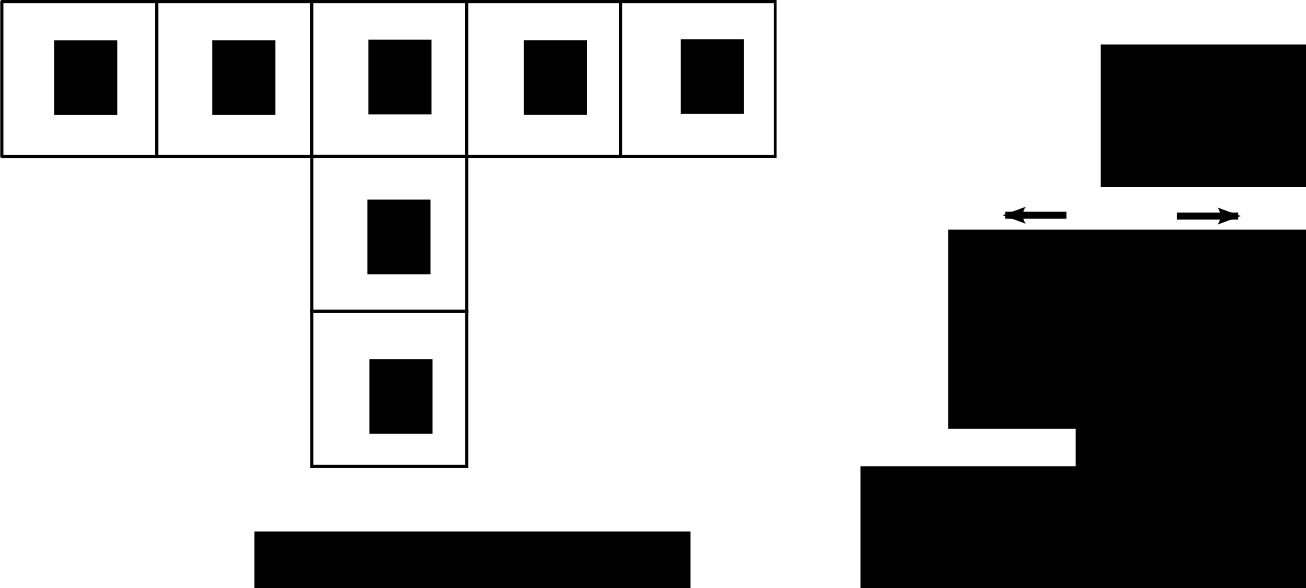
\includegraphics[width=\tworldsize\columnwidth]{\visualspdf/worlds_and_datasets/Tworld_with_state_number_and_action.pdf}
  \caption{The T world and the available actions.}
  \label{fig:Tworld}
\end{figure}

A simulated teacher wants the robot to reach the left edge of the T world. To this end, he will provide feedback information to the robot. Feedback signals are represented as two dimensional feature vectors and can have two different meanings: ``correct'' or ``incorrect''. In our example, as depicted in Figure~\ref{fig:feedbacksignals} those signals are randomly generate by two multivariate normal distribution, one for each meaning. When the teacher wants to send a feedback of meaning ``correct'', he will send a signals on the right part of the feature space. Respectively, for a feedback meaning ``incorrect'' the signal will be on the left side of the feature space. Those signals could represent any modality the teacher uses to communicate with the robot, such as speech, gestures, facial expression, or event brain signals. 

\begin{figure}[!htbp]
  \centering
  \includegraphics[width=\signalwidth\columnwidth]{\visualspdf/worlds_and_datasets/feedback_signals_color.pdf}
  \caption{The feedback signals used by our simulated teacher in our visual examples. A signal of meaning ``correct'' will be at the right side of the feature space, and a signal of meaning ``incorrect'' will be on the left side. Importantly, the agent will never have access to the label information.}
  \label{fig:feedbacksignals}
\end{figure}

The interaction between the agent and the teacher follow a turn-taking social behavior, and goes as follow. First, the agent, which is a particular state, performs one action and ends up in a new state. The teacher, which observes the scene evaluate this action with respect to the task he has in mind, and he sends a signal to the robot corresponding to the chosen meaning. However, the robot neither has access to the task the user has in mind, neither it has access the the meaning of the signal sent by the teacher.

For example, as depicted in Figure~\ref{fig:TworldOneStepUnlabeled}, the agent starts in state 3, performs action left, and ends-up in state 2. The teacher wants the agent to go to G1, therefore he sends a signal meaning that the previous action was ``correct'' with respect to the goal.

\begin{figure}[!htbp]
  \centering
  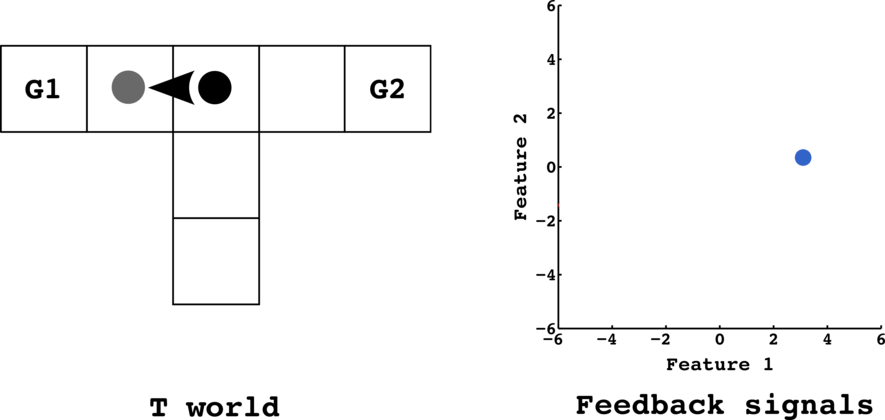
\includegraphics[width=\tworldsize\columnwidth]{\visualspdf/tuto_feedback/Tworld_feedback_unlabeled_one_action.pdf}
  \caption{The user provide a feedback signal after each action of the agent. The agent starts in state 3, performs action left, and ends-up in state 2. The teacher wants the agent to go to G1, therefore he sends a signal meaning that the previous action was ``correct'' with respect to the goal. Note that the signal is on the right side of the space as described in Figure~\ref{fig:feedbacksignals}. However the agent does not have access to the label associated to this signal and it only observes a point in a two dimensional space.}
  \label{fig:TworldOneStepUnlabeled}
\end{figure}

This sequence of interaction is repeated for several iteration until the agent agent finds out what the user wants it to do. After performing many actions, the robot ends-up with a lot of observations associating a state, an action and a feedback signal. As depicted in Figure~\ref{fig:TworldManyStepUnlabeled}, we can observe that two clusters has emerged in the feature space, this property will be exploited in the coming sections.

\begin{figure}[!htbp]
  \centering
  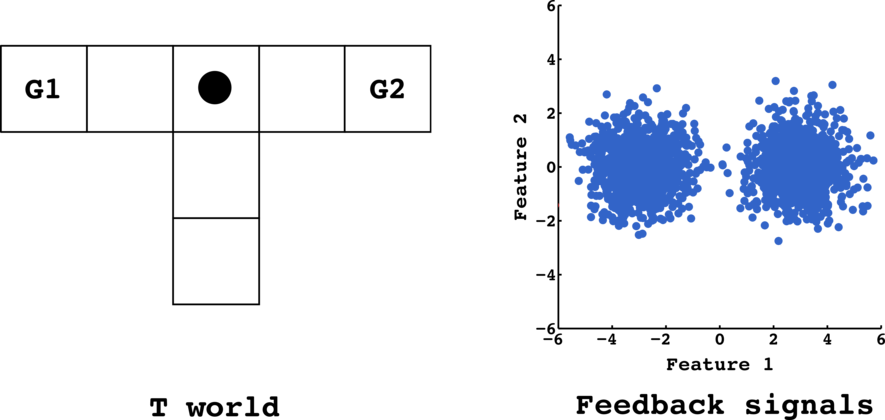
\includegraphics[width=\tworldsize\columnwidth]{\visualspdf/tuto_feedback/Tworld_feedback_unlabeled.pdf}
  \caption{After performing many actions, the robot ends-up with a lot of observations associating a state, an action and a feedback signal. The robot do not have access to the label associated to the teaching signals. However it can observe the distribution of signal in the feature space. We can observe that two clusters has emerged in the feature space, this property will be exploited in the coming sections.}
  \label{fig:TworldManyStepUnlabeled}
\end{figure}

\transition

This problem is impossible to solve without further information. In practice it would be easier if the robot had access to the mapping between teaching signals and their meanings. A usual solution is therefore to rely on a phase of calibration, where the system is given signal-meaning pairs and learn the mapping using supervised learning algorithm. Given this information, in our example of Figure~\ref{fig:TworldOneStepUnlabeled}, it becomes trivial to identify the task. Starting in state 3, if the robot do action ``left'', it ends up in state 2, and if it receives a signal of meaning ``correct'', then the correct task is to reach the left edge of the T marked by G1.

As mentioned before, in this work the robot does not have access to this information, neither it can rely on the phase of calibration. However the robot has access to theoretical information about the human teaching behavior. The robot knows that in a given situation, and for a particular task, the human should send a signal of a specific meaning. For example, the robot knows that if it moves from state 3 to state 4, and that the human wants it to go in G1, then the signals received from the human means ``incorrect''. Respectively, if the robot moves from state 3 to state 4, and that the human wants it to go in G2, then the signals received from the human means ``correct''.

The problem we want to solve resumes in trying to learn what to do without knowing the details of what we are told to do. We call this kind of problem learning from unlabeled interaction frame. 

\subsection{Learning from unlabeled interaction frame}

In previous chapter~\ref{chapter:humanexperiment:frames}, we defined the terms of interaction frames which represents a stereotyped situations, a schema of interpretation given a particular situation or event. Such frame is often assumed to be known by both the human and the robot in addition to the signal-to-meaning classifier that translate the actual human signals into meaningful symbols. By comparing what the frame predicts and what the human actually said the robot can change our understanding of the situation.

Learning from unlabeled interaction frames correspond to the problem where the signal-to-meaning classifier is not given, and therefore the robot can not rely on a direct comparison between the prediction from the interaction frame and the observation from the human teacher. 

What remains is the frame. It is at the core of our approach, it is assumed to be known by both the human and the robot. It includes both the constraints related to the task, e.g. teaching a robot which state to reach among a finite set of states, and the protocol used by the teacher to communicate to the robot, e.g. the teacher is assessing the robot's actions. Therefore, the meanings of the unlabeled signals is not explicitly given but is known to belong to a finite set of possible meanings.

We define a generic frame function that, given a context of interaction and a task, returns the meaning intended by the teacher:
%
\begin{eqnarray}
Meaning = Frame(Context, Task)
\end{eqnarray}
%
Following our previous example, stating that if the robot moves from state 3 to state 4 (context), and that the human wants it to go in G1 (task), then the signals received from the human means ``incorrect'' (meaning), we can exemplify the use of the frame:
%
\begin{eqnarray}
``incorrect" = Frame((s3 \rightarrow s4), G1)
\end{eqnarray}

\transition

The idea of unlabeled interaction frame summarizes the problem of interaction we tackle in this work. However it is a quite general concept, and in order to understand the underlying principles of our algorithm, in the following sections we will restrict our analysis to simple frames and simple worlds. We will also explicit a number of assumptions related to this work.


%%%%%%%%%%%%%%%%%%%%%%%%%%%%%%%%%%%%%%%%%%%%%%
%%%%%%%%%%%%%%%%%%%%%%%%%%%%%%%%%%%%%%%%%%%%%%
%%%%%%%%%%%%%%%%%%%%%%%%%%%%%%%%%%%%%%%%%%%%%%
%%%%%%%%%%%%%%%%%%%%%%%%%%%%%%%%%%%%%%%%%%%%%%
%%%%%%%%%%%%%%%%%%%%%%%%%%%%%%%%%%%%%%%%%%%%%%
\section{What do we exploit}

In this section, we present small visual representations of the problem showing what properties can be exploited. As detailed before, we assume the robot knows about the frame of interaction. 

Following our example in section~\ref{chapter:lfui:example}, the robot knowns the world, the effect of it actions. The robot also knows the human wants it to reach one of the two edges of the T world marked with G1 and G2. The robot is also aware of the interaction frame, in our case that the teacher will provide, for each action performed by the robot, a feedback signal meaning either ``correct'' or ``incorrect''. The robot further knows how the teacher should behave with respect to one particular goal.

Central to our method is a system of hypothesis. From the observation made in chapter~\ref{chapter:humanexperiment:interpretationhypothesis}, with the available information, the robot will generate interpretation hypothesis with respect to all possible tasks. For a particular hypothesis, the robot will assign hypothetic meanings to the human signals knowing their are limited to a fixed set and according to the current state of the world. The machine is ``reasoning'' as follow: \emph{"If the human wants me to solve task G1 then when I performed action ``right'' in state $3$, its feedback signal means ``incorrect''"}. 

We exemplify the idea of interpretation hypothesis following our T world example in section~\ref{chapter:lfui:example}. For the sake of our example, we only consider two hypothesis, G1 and G2, as depicted in Figure~\ref{fig:TworldManyStepUnlabeled}.

\subsection{Interpretation hypothesis}
\label{chapter:lfui:interpreation}

We considerer the same interaction as in section~\ref{chapter:lfui:example}. For each action, the robot receives raw unlabeled two dimensional signals. For the sake of the example and ease of explanation, we consider those two-dimensional signals as representing speech utterances.

Following the above explanation, for a particular hypothesis (G1 or G2), the robot can assign hypothetic meanings to the human signals knowing their are limited to a fixed set and according to the current state of the world. The machine is ``reasoning'' as follow: \emph{"If the human wants me to solve task G1 then when I performed action $a$ in state $a$ and he said ``oui'', he meant ``incorrect''"}. 

We exemplify this process using the same example as in Figure~\ref{fig:TworldOneStepUnlabeled} and according to our two task hypothesis which are reaching either of the two edges marked as G1 or G2. The robot is aware of the optimal policies (see Figure~\ref{fig:Twolrdpolicies}) for each task which it can use to interpret the human signals.

\begin{figure}[!htbp]
  \centering
  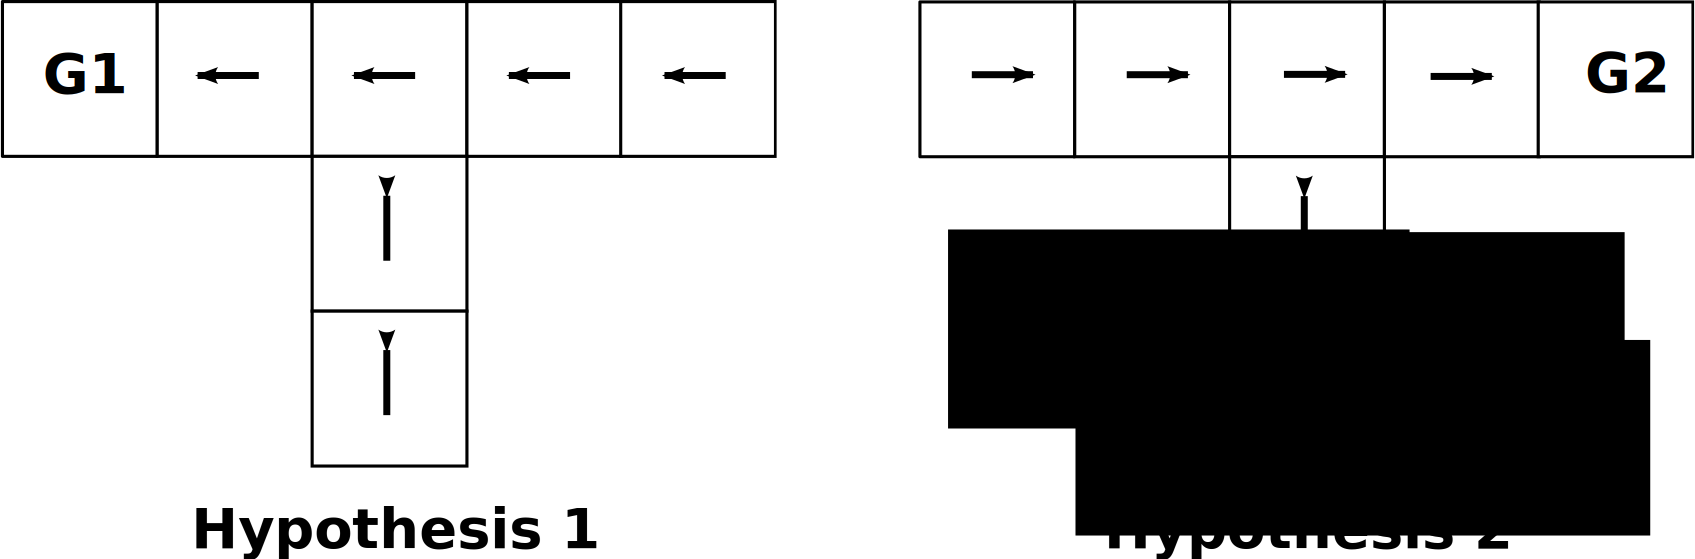
\includegraphics[width=\tworldsize\columnwidth]{\visualspdf/tuto_feedback/Tworld_hypothesis.pdf}
  \caption{Optimal policies associated to the two task hypothesis G1 and G2 in the T world. Such policies are known by both the human and the agent, and allow the agent to interpret a human signal with respect to a given task.}
  \label{fig:Twolrdpolicies}
\end{figure}

The agent starts in state 3, performs action left, and ends-up in state 2. The teacher wants the agent to go to G1, therefore he sends a signal meaning that the previous action was ``correct'' with respect to the goal. However the agent does not have access to the label associated to this signal and it only observes a point in a two dimensional space. The agent will therefore generate interpretation hypothesis according to G1 and G2. With respect to the G1, the action was ``correct'' (Figure~\ref{fig:TworldLabelG1}) while with respect to G2 the action was ``incorrect'' (Figure~\ref{fig:TworldLabelG1}).

\begin{figure}[!htbp]
    \centering
    \begin{subfigure}[b]{\tworldsize\columnwidth}
        \centering
        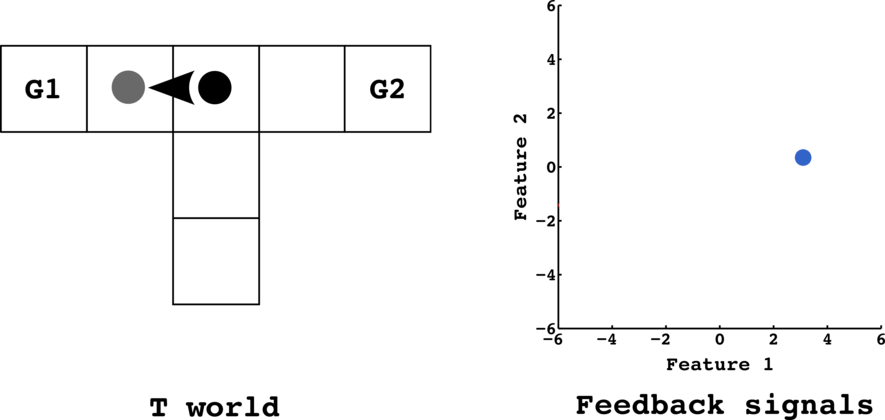
\includegraphics[width=\columnwidth]{\visualspdf/tuto_feedback/Tworld_feedback_unlabeled_one_action.pdf}
        \caption{Feedback signal as received by the agent without label.}
    \end{subfigure}\\
    \begin{subfigure}[b]{\tworldsize\columnwidth}
        \centering
        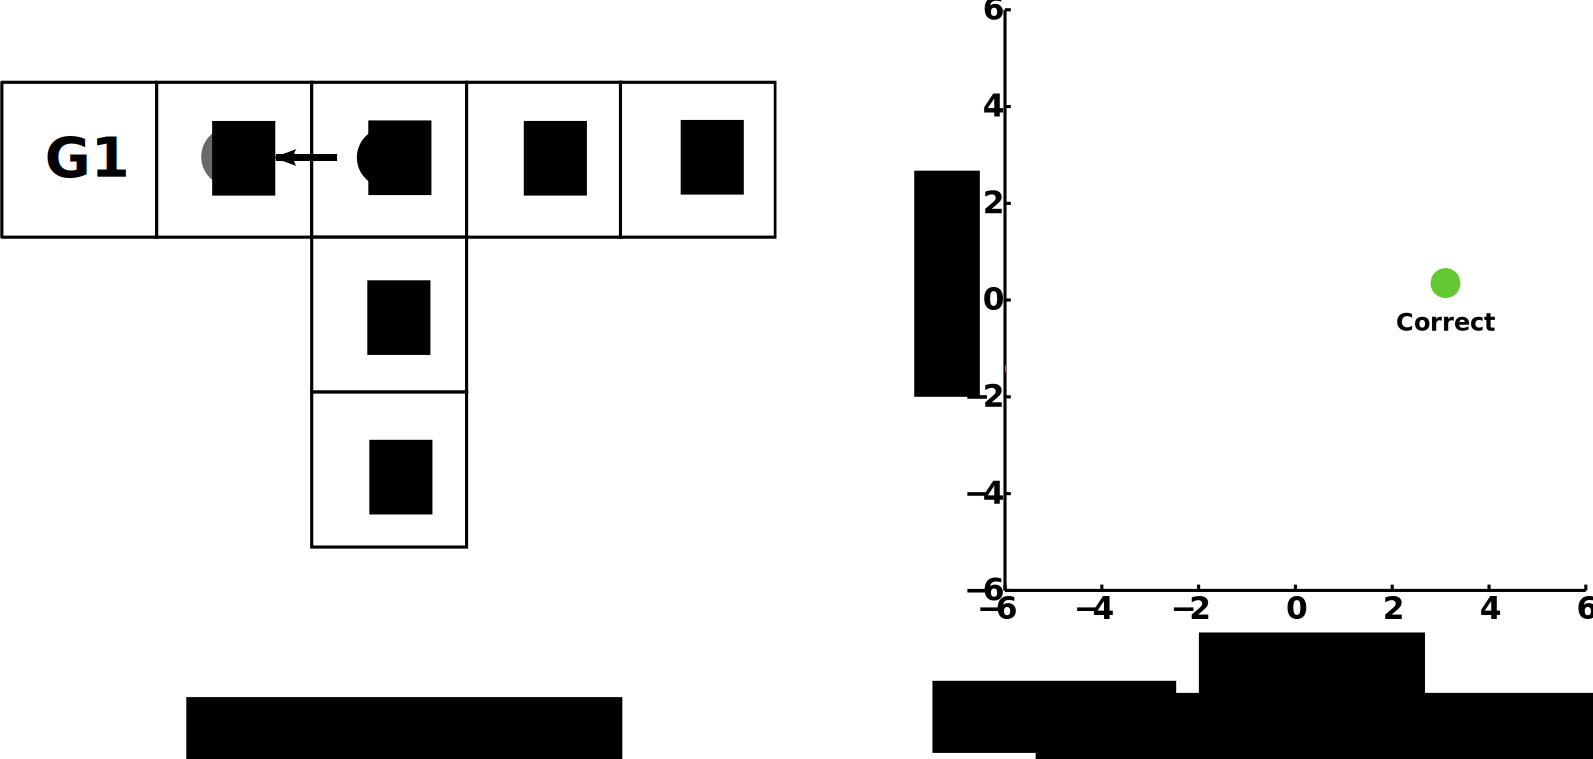
\includegraphics[width=\columnwidth]{\visualspdf/tuto_feedback/Tworld_feedback_labeled_G1.pdf}
        \caption{Feedback signal labeled according to G1.}
        \label{fig:TworldLabelG1}
    \end{subfigure}
    \begin{subfigure}[b]{\tworldsize\columnwidth}
        \centering
        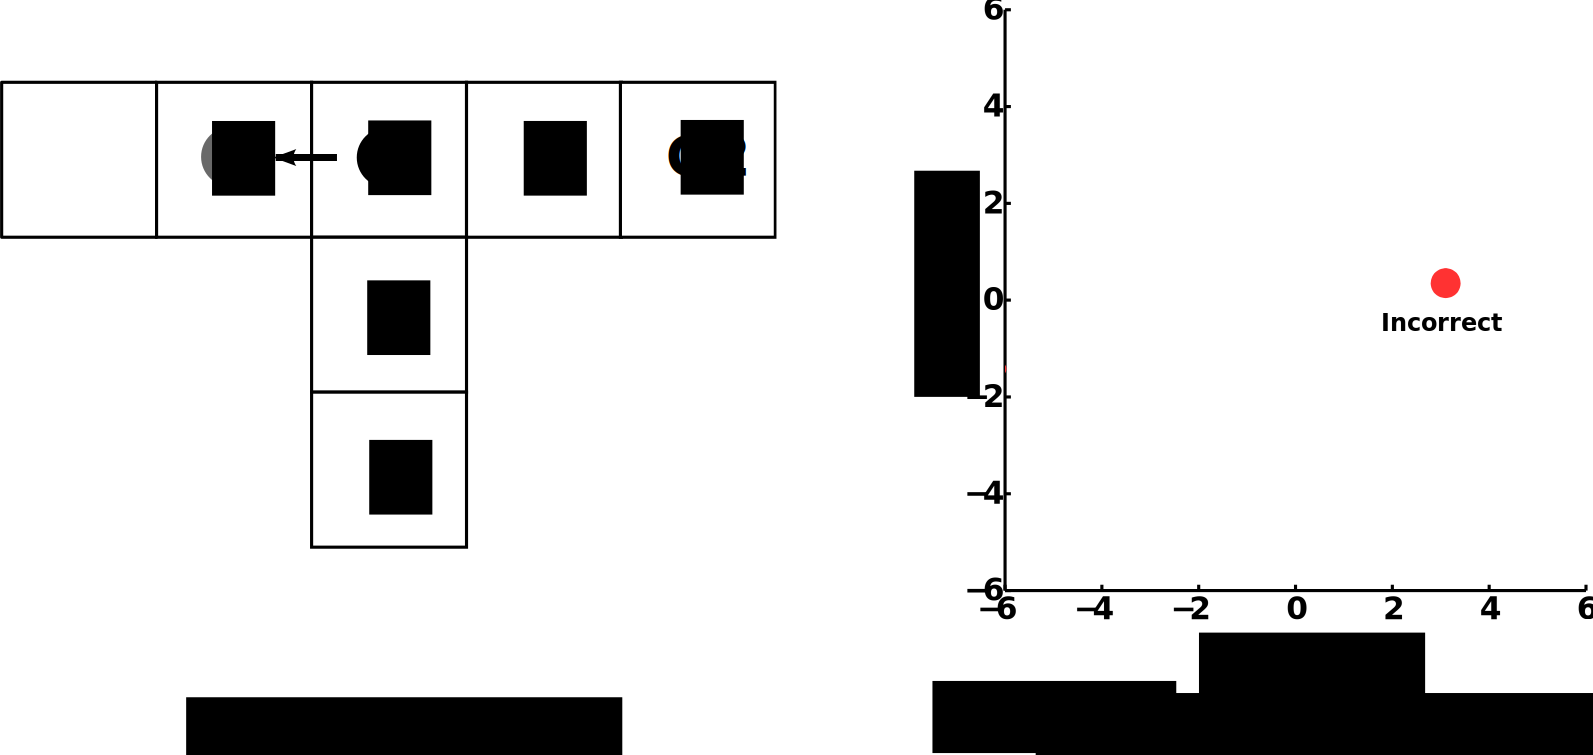
\includegraphics[width=\columnwidth]{\visualspdf/tuto_feedback/Tworld_feedback_labeled_G2.pdf}
        \caption{Feedback signal labeled according to G2.}
        \label{fig:TworldLabelG2}
    \end{subfigure}
    \caption{Interpretation hypothesis made by the agent according to G1 (\ref{fig:TworldLabelG1}) and G2 (\ref{fig:TworldLabelG2}). The agent starts in state 3, performs action left, and ends-up in state 2. The meaning of the signal is different in both for both hypothesis.}
    \label{fig:TworldLabelOneStep}
\end{figure}

By repeating this process for several iteration steps with the agent exploring all possible state-action pair, the system end-up with a set of possible interpretation of the human teaching signals. But as the user have only one objective in mind, here G1, only the correct interpretation will exhibit a coherence between the signals and their associated meanings. Note that when the agent moves in the trunk of the T, the interpretation hypothesis with respect to G1 an G2 give the same labels. Details about this interaction will be given in chapter~\ref{chapter:planning} to explain the problem of planning, here we assume the robot explores all state-action.

\begin{figure}[!htbp]
    \centering
    \begin{subfigure}[t]{\tworldsize\columnwidth}
        \centering
        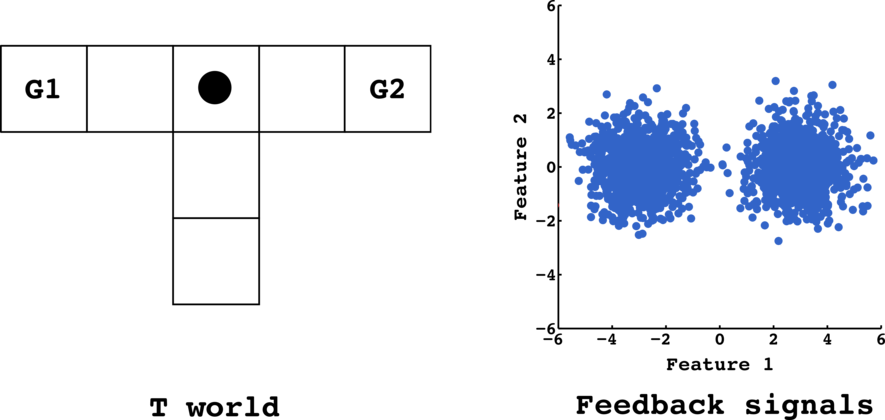
\includegraphics[width=\columnwidth]{\visualspdf/tuto_feedback/Tworld_feedback_unlabeled.pdf}
        \caption{Feedback signal as received by the agent without label.}
    \end{subfigure}\\
    \begin{subfigure}[b]{\columnwidth}
        \centering
        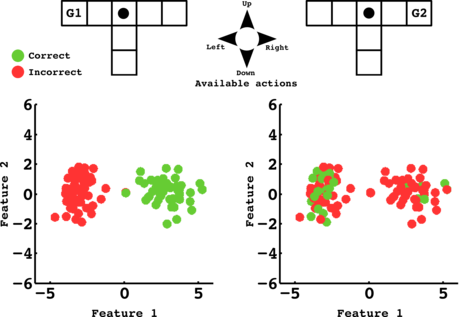
\includegraphics[width=\columnwidth]{\visualspdf/tuto_feedback/Tworld_feedback_labeled_all_actions.pdf}
        \caption{Feedback signal labeled according to G1 and G2.}
        \label{fig:TworldLabelinterpretation}
    \end{subfigure}
    \caption{Interpretation hypothesis made by the agent according to G1 and G2 after many interaction steps. The teacher's task is to have the agent reach G1. The agent is exploring all the state space randomly. The labels associated to the task G1 are more coherent with the spacial organization of signals in the feature space.}
    \label{fig:TworldLabel}
\end{figure}

In our case, as we assume the user is coherent and uses always the same kind of signal for the same meaning. By visual inspection, we can infer that hypothesis G1 is the correct one as the resulting mapping between signal and meaning is more coherent. The key challenge now is it find out how to identify a coherence between the spacial organization of label in the feature space and their associated labels with the tools available to the robot. We will formalize this idea in section \ref{chapter:lfui:how}. 

\subsection{Different frames}

We have seen the feedback frames where the human user is assessing the robot action. In this thesis, we will also consider a different interaction frame, where the user would indicate the robot which action to perform next. We call this kind of interaction frame the guidance frame.

We will give several visual example of the guidance frame in the following of this chapter.

% , we simply illustrate here the signal that will be associated to the different action. As depicted in Figure~\ref{fig:guidancesignals}, we used an easy to remember way of presenting the data, the cluster at the top of the feature space represents the ``up'' action, the one at the bottom the ``down'' action, the one at the right the ``right'' action, and the one at the left the ``left'' action.

% \begin{figure}[!htbp]
%   \centering
%   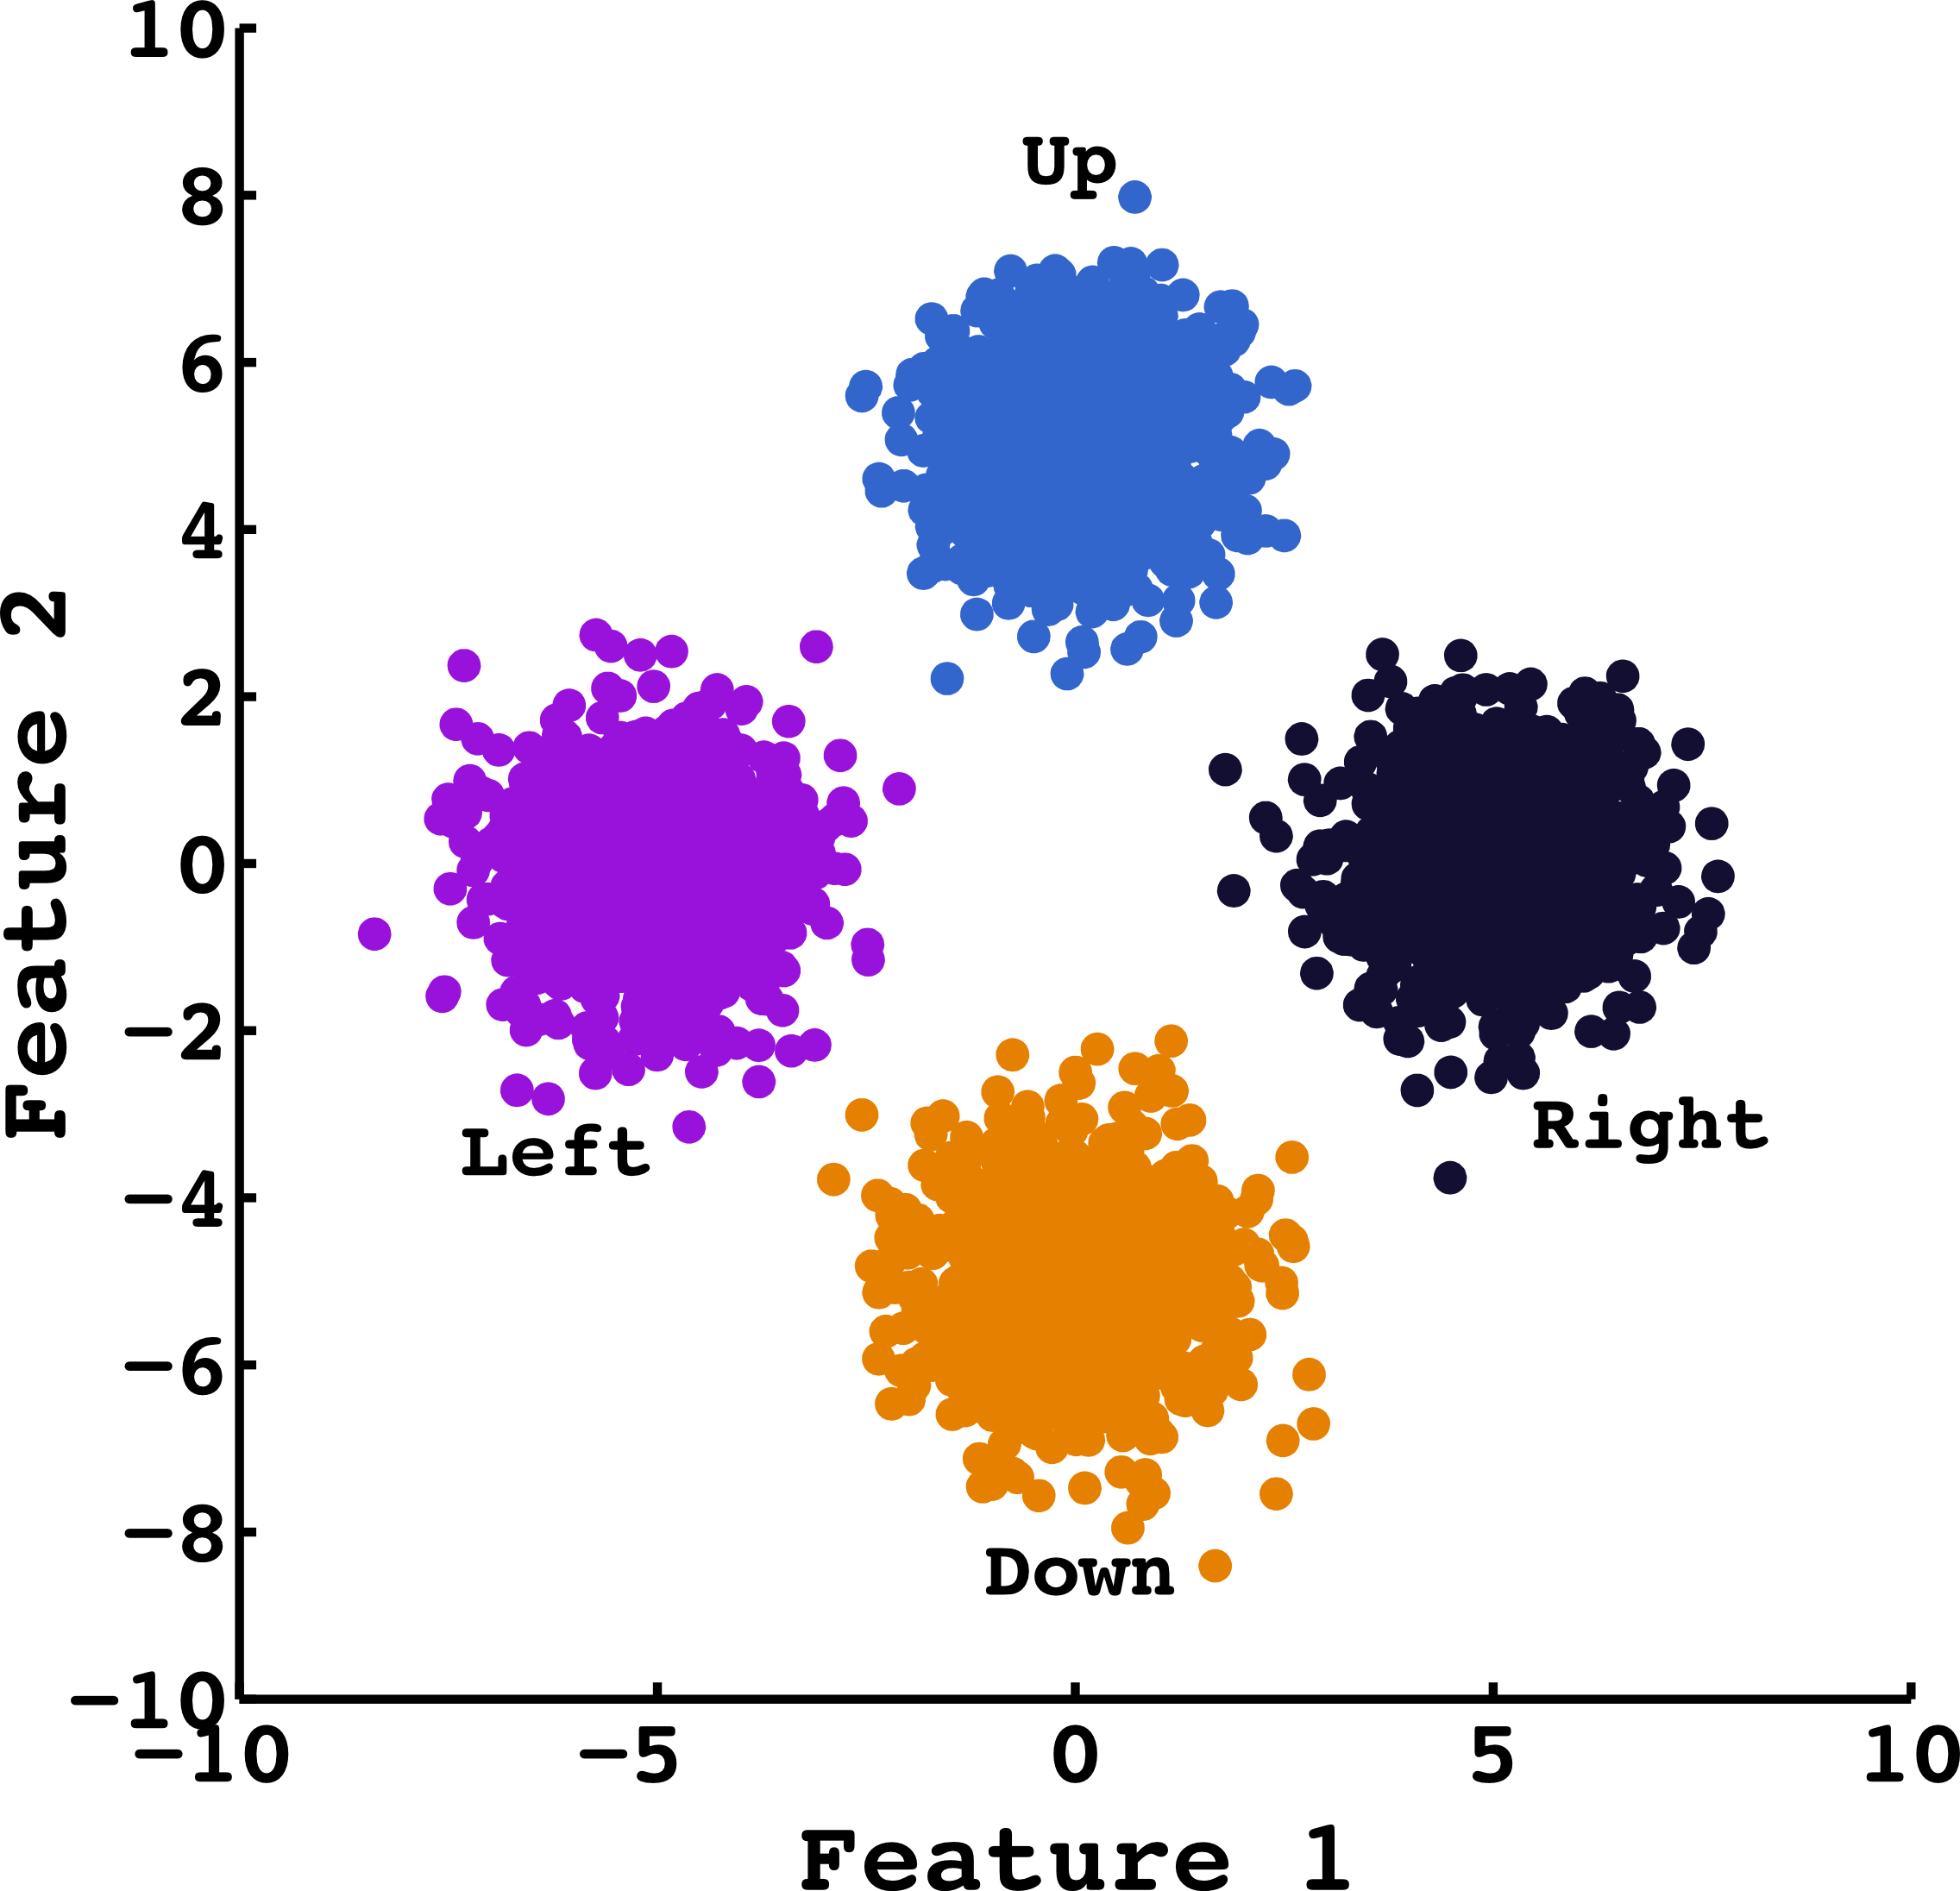
\includegraphics[width=\signalwidth\columnwidth]{\visualspdf/worlds_and_dataset/guidance_4_signals_color.pdf}
%   \caption{The guidance signals used by our simulated teacher in our visual examples.}
%   \label{fig:guidancesignals}
% \end{figure}

\subsection{Why not a clustering algorithm}
\label{chapter:lfui:whynotEM}

When we first look at the unlabeled signals, the first approach that one as in mind is to use a clustering algorithm to find the two clusters in the feature space. For very simple dataset, like the one presented in Figure~\ref{fig:TworldManyStepUnlabeled}, a clustering algorithm will find the two clusters. However, without any additional information, it is impossible to know which one is associated to the meaning ``correct'' or to the meaning ``incorrect''.

More importantly, clustering algorithms are prone to local extrema in the optimization process and for those datasets in high dimension with overlapping classes it is unlikely to find the correct underlying structure of the data. Our approach has the advantage to have access to hypothetic labels allowing to fit a classifier for each task hypothesis.

%%%%%%%%%%%%%%%%%%%%%%%%%%%%%%%%%%%%%%%%%%%%%%
%%%%%%%%%%%%%%%%%%%%%%%%%%%%%%%%%%%%%%%%%%%%%%
%%%%%%%%%%%%%%%%%%%%%%%%%%%%%%%%%%%%%%%%%%%%%%
%%%%%%%%%%%%%%%%%%%%%%%%%%%%%%%%%%%%%%%%%%%%%%
%%%%%%%%%%%%%%%%%%%%%%%%%%%%%%%%%%%%%%%%%%%%%%
\section{Assumptions}
\label{chapter:lfui:assumptions}

As depicted before a number of assumptions are made on the information accessible to the robot and the constraints applied on the interaction.

\subsection{Frames}

The first assumption is that the robot and the human are aware of the frame in which the interaction take place. This frame regulates the interaction between the two partners, it includes:

\begin{itemize}

\item \textbf{The set of possible meanings the human can refer to.} As depicted before, the set of meaning includes ``correct'' and ``incorrect'' for thoses cases where the user is assessong te robot's actions. It could also be the set of action names for those case where the user provides guidance on what to do next.

\item \textbf{Details and timing of the interaction:} it corresponds to when and how the user will provide instruction signals. For example, the human sends a signal to the robot after each action the robot performs. An other example may be the human providing a feedback signal between 0.2 and 2 seconds after the robot's action he is referring to, like in \cite{knox2009interactively}.

\item \textbf{Constraints on the possible tasks:} For example the robot is aware that the human wants to have it grasp one object on the table. And not reach for an object in a different room. This limits the number of hypothesis the robot can create.

\end{itemize}

By combining those three aspect of an interaction frame, the robot can create a set of interpretation hypothesis for the received teaching signals. For one possible task, and given a specific context (e.g. state and action performed in the environment), the robot can infer the meaning intended by the human user. By doing so for each possible task, it creates a set of interpretation hypothesis, which we rely on to fond the task taught by the user, as well as the signal to meaning mapping.

To do so we rely on specific properties of the human teaching signals.

\subsection{Signals properties}
\label{chapter:lfui:signalproperties}

We make two assumptions about the human teaching signals properties:
\begin{itemize}

\item If the true intended meaning associated to each user signal was known it would be possible to train a classifier with reasonable accuracy. We will see in chapter~\ref{chapter:planning:results} that the performance of the system are highly impacted by the quality of the training data.

\item The teacher is coherent in its use of teaching signals and will always use the name kind of signals to mean the same things. For the case of two buttons, he will always use the same button to mean the same thing. It also apply for speech, facial expression, gestures, or brain signals. 

\end{itemize}

Those two properties are usual assumption in human-robot interaction, we here simply assume we can rely on the teacher behavior and that we could, in theory, learn a signal to meaning mapping.

However there is one practical constraint that differ from more standard human-robot interaction scenario. Here, in theory, we cannot know in advance if a signal to meaning mapping can be learn. Indeed we do not have access to a database of signal-meaning pairs to train a classifier first, which allow to try different feature extraction process or different classifiers beforehand. This limitation requires to ensure the representation of the signal as well as the selected classifier allow to learn a signal to meaning mapping. 

We will see from results in chapter~\ref{chapter:planning:results} that our algorithm can cope with highly overlapping data where the classifier produce close to random prediction. In such cases the algorithm will not make decision on which task is the correct one.

\subsection{World properties and symmetries}
\label{chapter:lfui:symmetries}

There is come cases where some hypothesis are not distinguishable. As the robot do not have a direct access to the true intended meaning of the user signals, it can only rely on the interpretation hypothesis made for each task.

Two problems could appear \begin{inparaenum}[a)] \item two hypothesis may share the same interpretation model and can not be differentiate as they will attribute the same meaning to the signals, and \item two hypothesis may end up with opposite interpretation that are both as valid. \end{inparaenum}.

For those case where two hypothesis share the same interpretation model, either the task are the same with respect the user, either some parts of the problem are hidden to the human user which can not provide instruction for them. We do not tackle this problematic in this thesis and assume the world properties ensure that two hypothesis will never share the same interpretation model. Most of the hypothesis will share some parts of the interpretation model but there will always exist one situation where two interpretation models separate.

For those case where two hypothesis end up with opposite interpretation that are both valid, we first present a small example showcasing the problem.

We present the line word in Figure~\ref{fig:lineworld} which contains only the top T bar of the T world. This world is very well suited to describe the symmetry problem. 

\begin{figure}[!htbp]
  \centering
  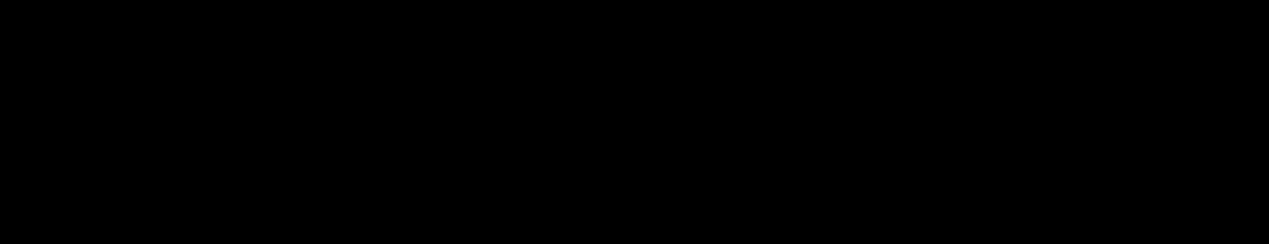
\includegraphics[width=\tworldsize\columnwidth]{\visualspdf/worlds_and_datasets/lineworld_with_state_number_and_2action.pdf}
  \caption{The line world and the available actions.}
  \label{fig:lineworld}
\end{figure}

The interaction follows the same protocol as in previous examples, and following the feedback frame. As depicted in Figure~\ref{fig:lineworldfeedback2action}, after several interaction steps, the interpretation hypothesis for G1 and G2 display symmetric properties. Indeed, even if in the end the interpretation of the signals differ between the hypothesis, the two interpretation match well with the data. As the optimal policies to reach each of the two goal states are symmetric in every state, the actions that trigger ``correct'' feedback with respect to G1 trigger ``incorrect'' feedback for G2 and vice versa. It is therefore impossible to know the true associated meaning of the signals without further information.

\begin{figure}[!htbp]
  \centering
  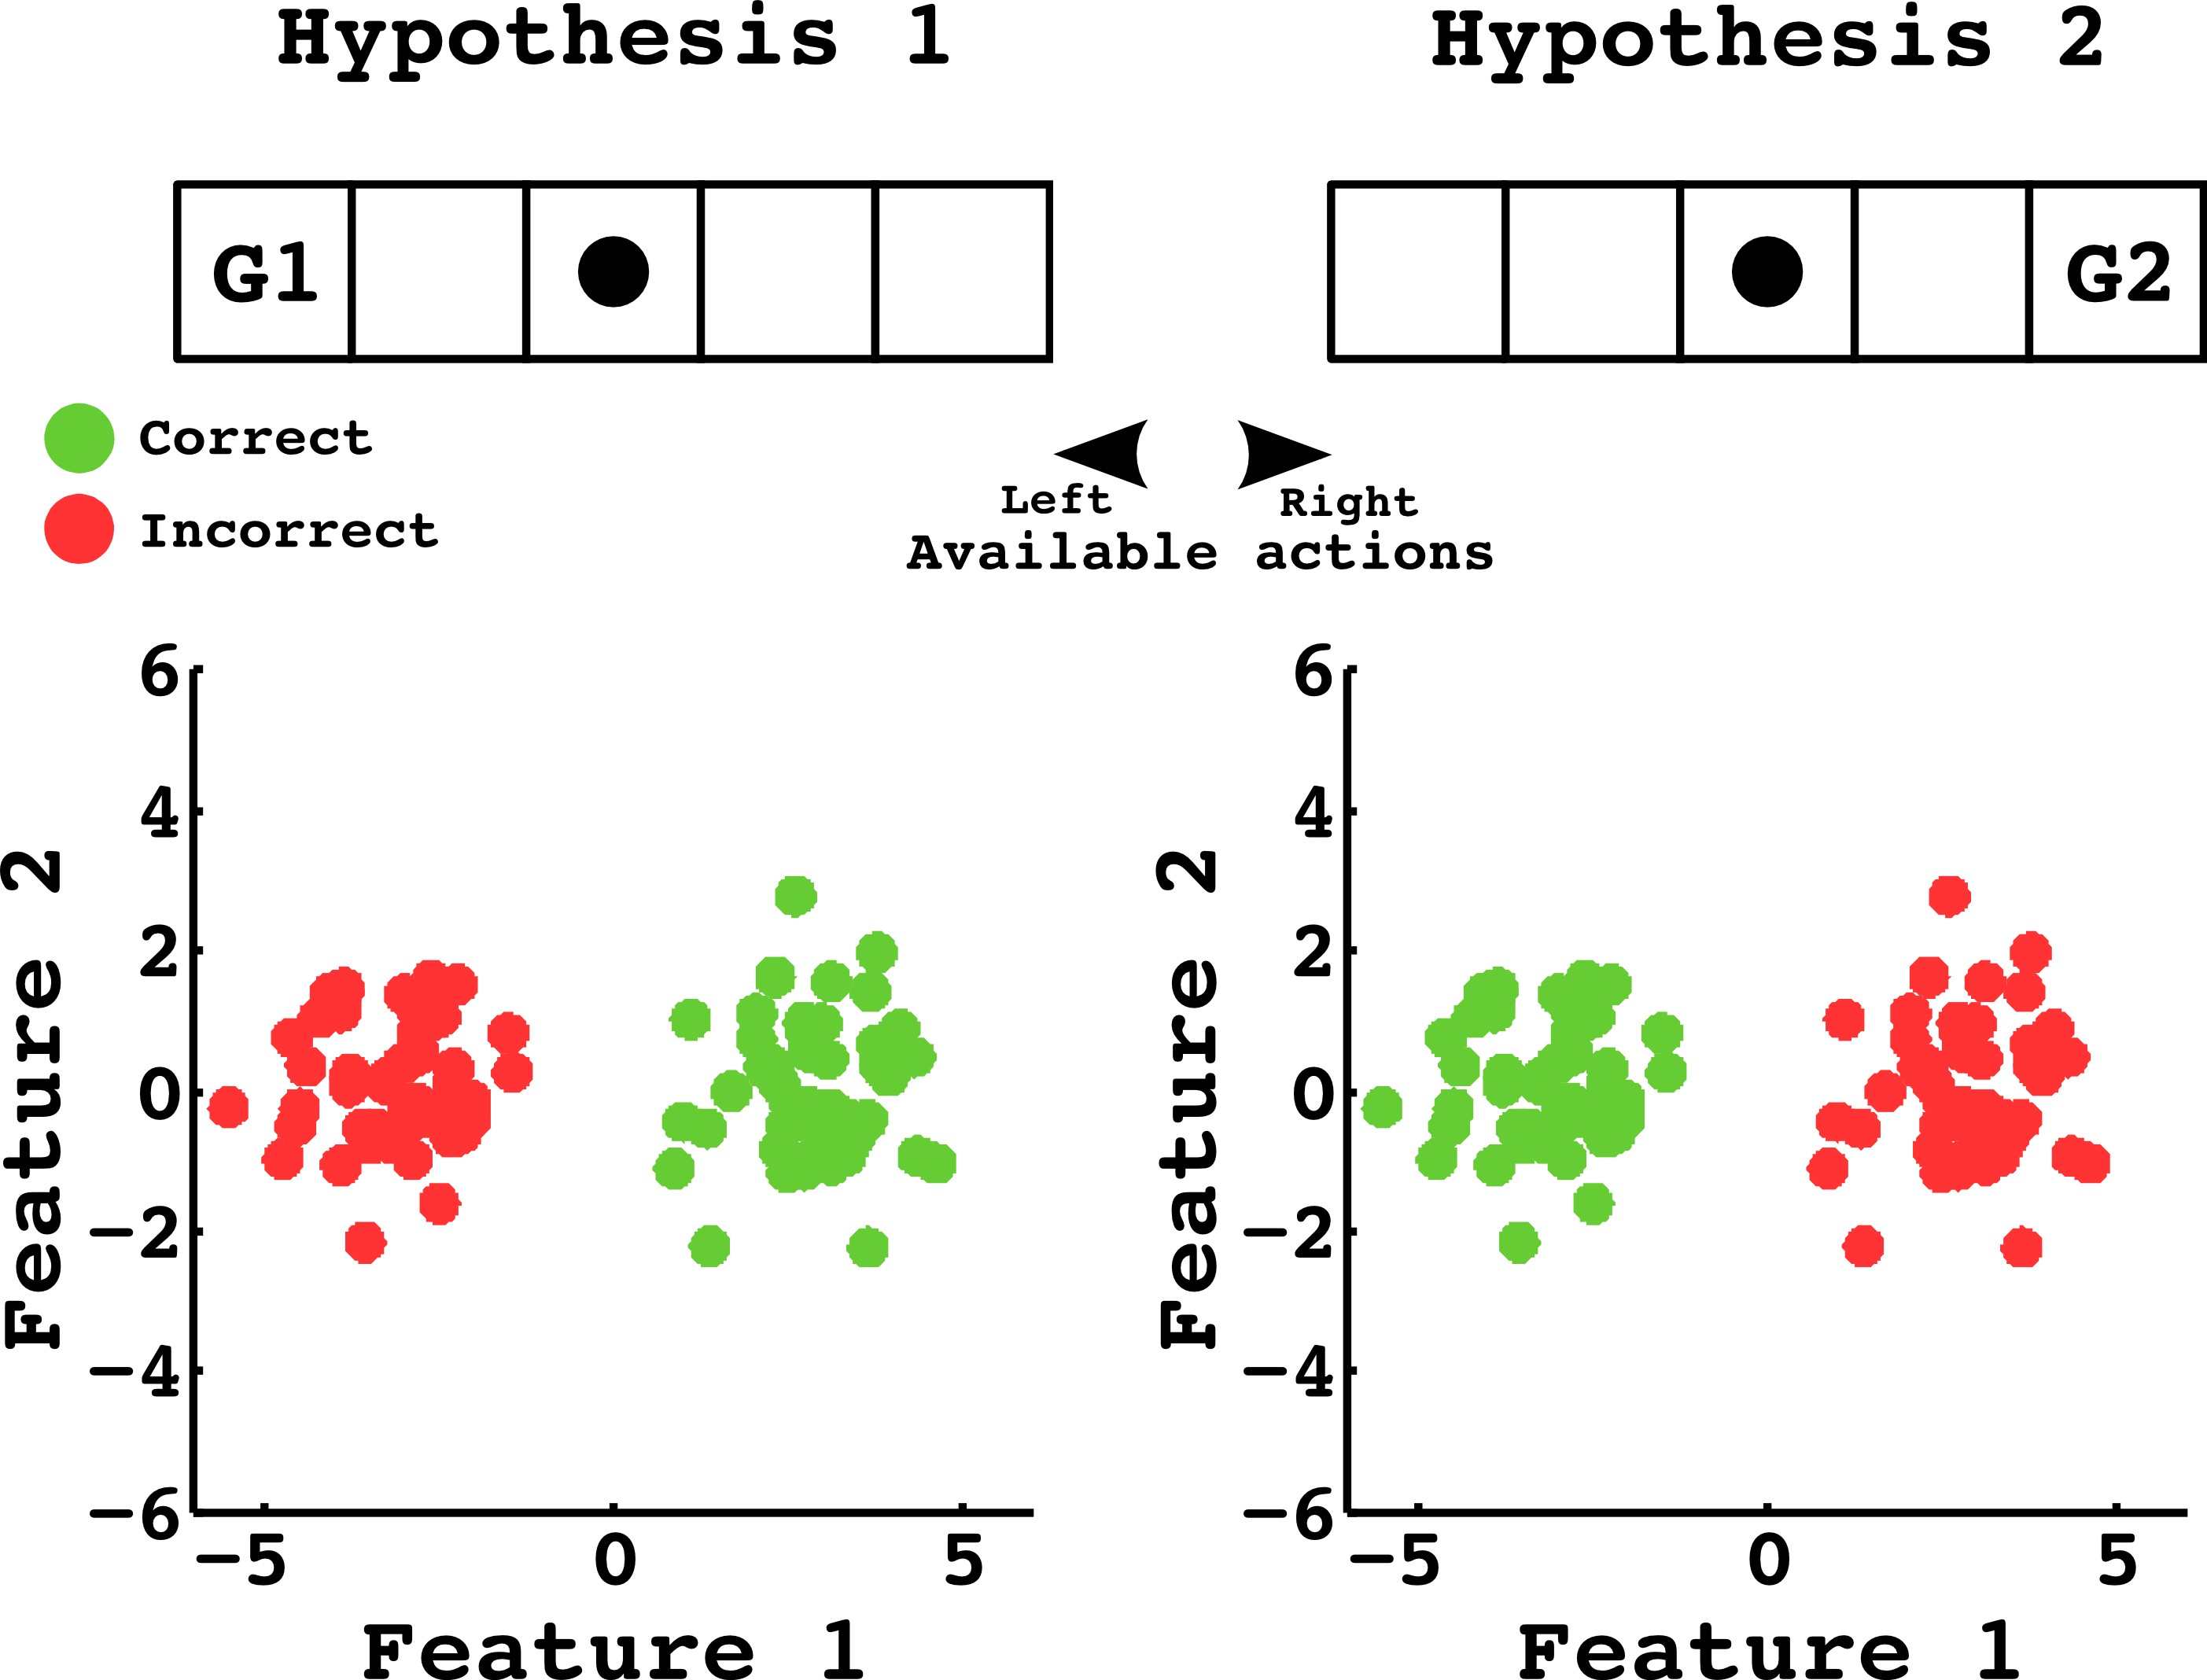
\includegraphics[width=\tworldsize\columnwidth]{\visualspdf/lineworld_symmetries/feedback_2actions.pdf}
  \caption{Interpretation hypothesis for an agent receive feedback on its action in the line word and where hypothetic task are G1 or G2. The agent can only perform right or left action which results in symmetric interpretation hypothesis of the feedback signals.}
  \label{fig:lineworldfeedback2action}
\end{figure}

It is theoretically impossible to differentiate symmetric task hypothesis, therefore we will not consider environments holding this symmetric properties. One way to solve this problem is to add a ``no move'' action that is valid only at the goal state, as depicted in Figure~\ref{fig:lineworld3action}.

\begin{figure}[!htbp]
  \centering
  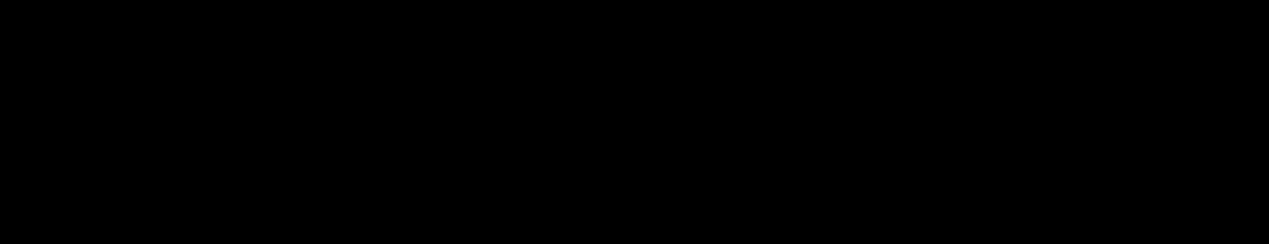
\includegraphics[width=\tworldsize\columnwidth]{\visualspdf/worlds_and_datasets/lineworld_with_state_number_and_action.pdf}
  \caption{The line world and the new available actions, including a ``no move'' action.}
  \label{fig:lineworld3action}
\end{figure}

When taking this action the agent to not change position on the grid. This action brakes the symmetry in the above example, as its interpretation will be the same for all states that are not an hypothetic goal state. In other words, in state 3, if agent performs action ``no move'', then the user will produce a signal meaning ``incorrect'', because the agent is neither in G1 nor in G2. And the signal will be interpreted as an ``incorrect'' by the two interpretation hypothesis, breaking the symmetry problem. The interpretation results after several iteration steps and using the new ``no move'' action are depicted in Figure~\ref{fig:lineworldfeedback3action}.

\begin{figure}[!htbp]
  \centering
  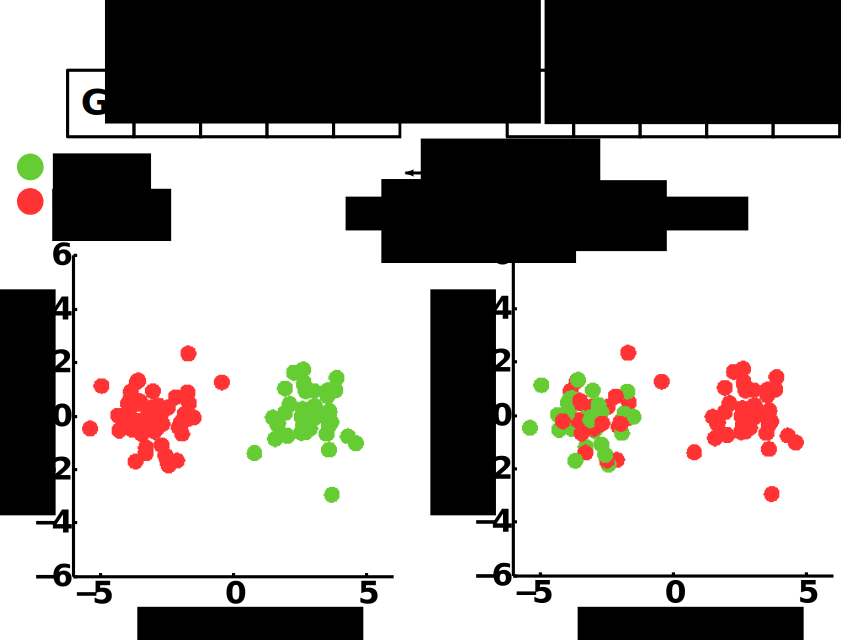
\includegraphics[width=\tworldsize\columnwidth]{\visualspdf/lineworld_symmetries/feedback_3actions.pdf}
  \caption{Interpretation hypothesis for an agent receive feedback on its action in the line word and where hypothetic task are G1 or G2. The agent can perform right, left, or a ``no move'' action. As opposed to Figure~\ref{lineworldfeedback2action}, the ``no move'' action allow to break the symmetry of interpretation between G1 and G2.}
  \label{fig:lineworldfeedback3action}
\end{figure}

This problem of symmetries holds for the guidance frame too. Indeed if the agent can only produce ``left'' and ``right'' commands, the interpretation hypothesis for G1 will be symmetric as the one for G2. If the user wants the robot to reach G1, it will only produce ``left'' guidance signals, which is represented by one cluster in the the feature space. And the ``right'' commands should never be used. The situation is symmetric for G2. The resulting interpretation hypothesis are shown in Figure~\ref{fig:lineworldguidance2action}.

\begin{figure}[!htbp]
  \centering
  \includegraphics[width=\signalwidth\columnwidth]{\visualspdf/worlds_and_datasets/guidance_2_signals_color.pdf}
  \caption{The guidance signals used by our simulated teacher in our line world visual examples with two actions.}
  \label{fig:lineworldguidance2signals}
\end{figure}

\begin{figure}[!htbp]
  \centering
  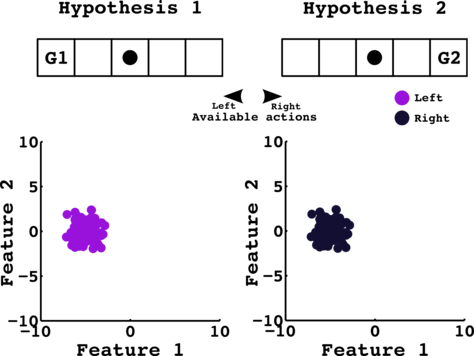
\includegraphics[width=\tworldsize\columnwidth]{\visualspdf/lineworld_symmetries/guidance_2actions.pdf}
  \caption{Interpretation hypothesis for an agent receive guidance on its action in the line word and where hypothetic task are G1 or G2. The agent can only perform right or left action which results in symmetric interpretation hypothesis of the guidance signals.}
  \label{fig:lineworldguidance2action}
\end{figure}

When introducing the ``goal reached'' action, the user now can produce three different kind of meanings, which is represented by three different clusters in the feature space. However, here again, one of the meaning won't be used by the teacher. However the ``goal reached'' signal will be used only at the goal space, which is not the same for the two hypothesis, which break the symmetry. The resulting interpretation hypothesis are shown in Figure~\ref{fig:lineworldguidance3action}.

\begin{figure}[!htbp]
  \centering
  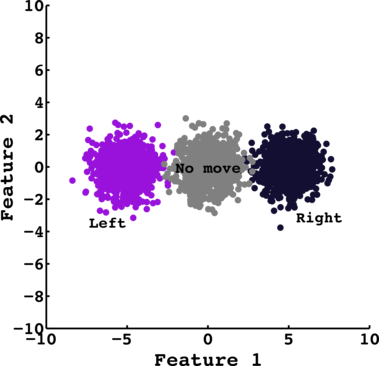
\includegraphics[width=\signalwidth\columnwidth]{\visualspdf/worlds_and_datasets/guidance_3_signals_color.pdf}
  \caption{The guidance signals used by our simulated teacher in our line world visual examples with three actions.}
  \label{fig:lineworldguidance3signals}
\end{figure}

\begin{figure}[!htbp]
  \centering
  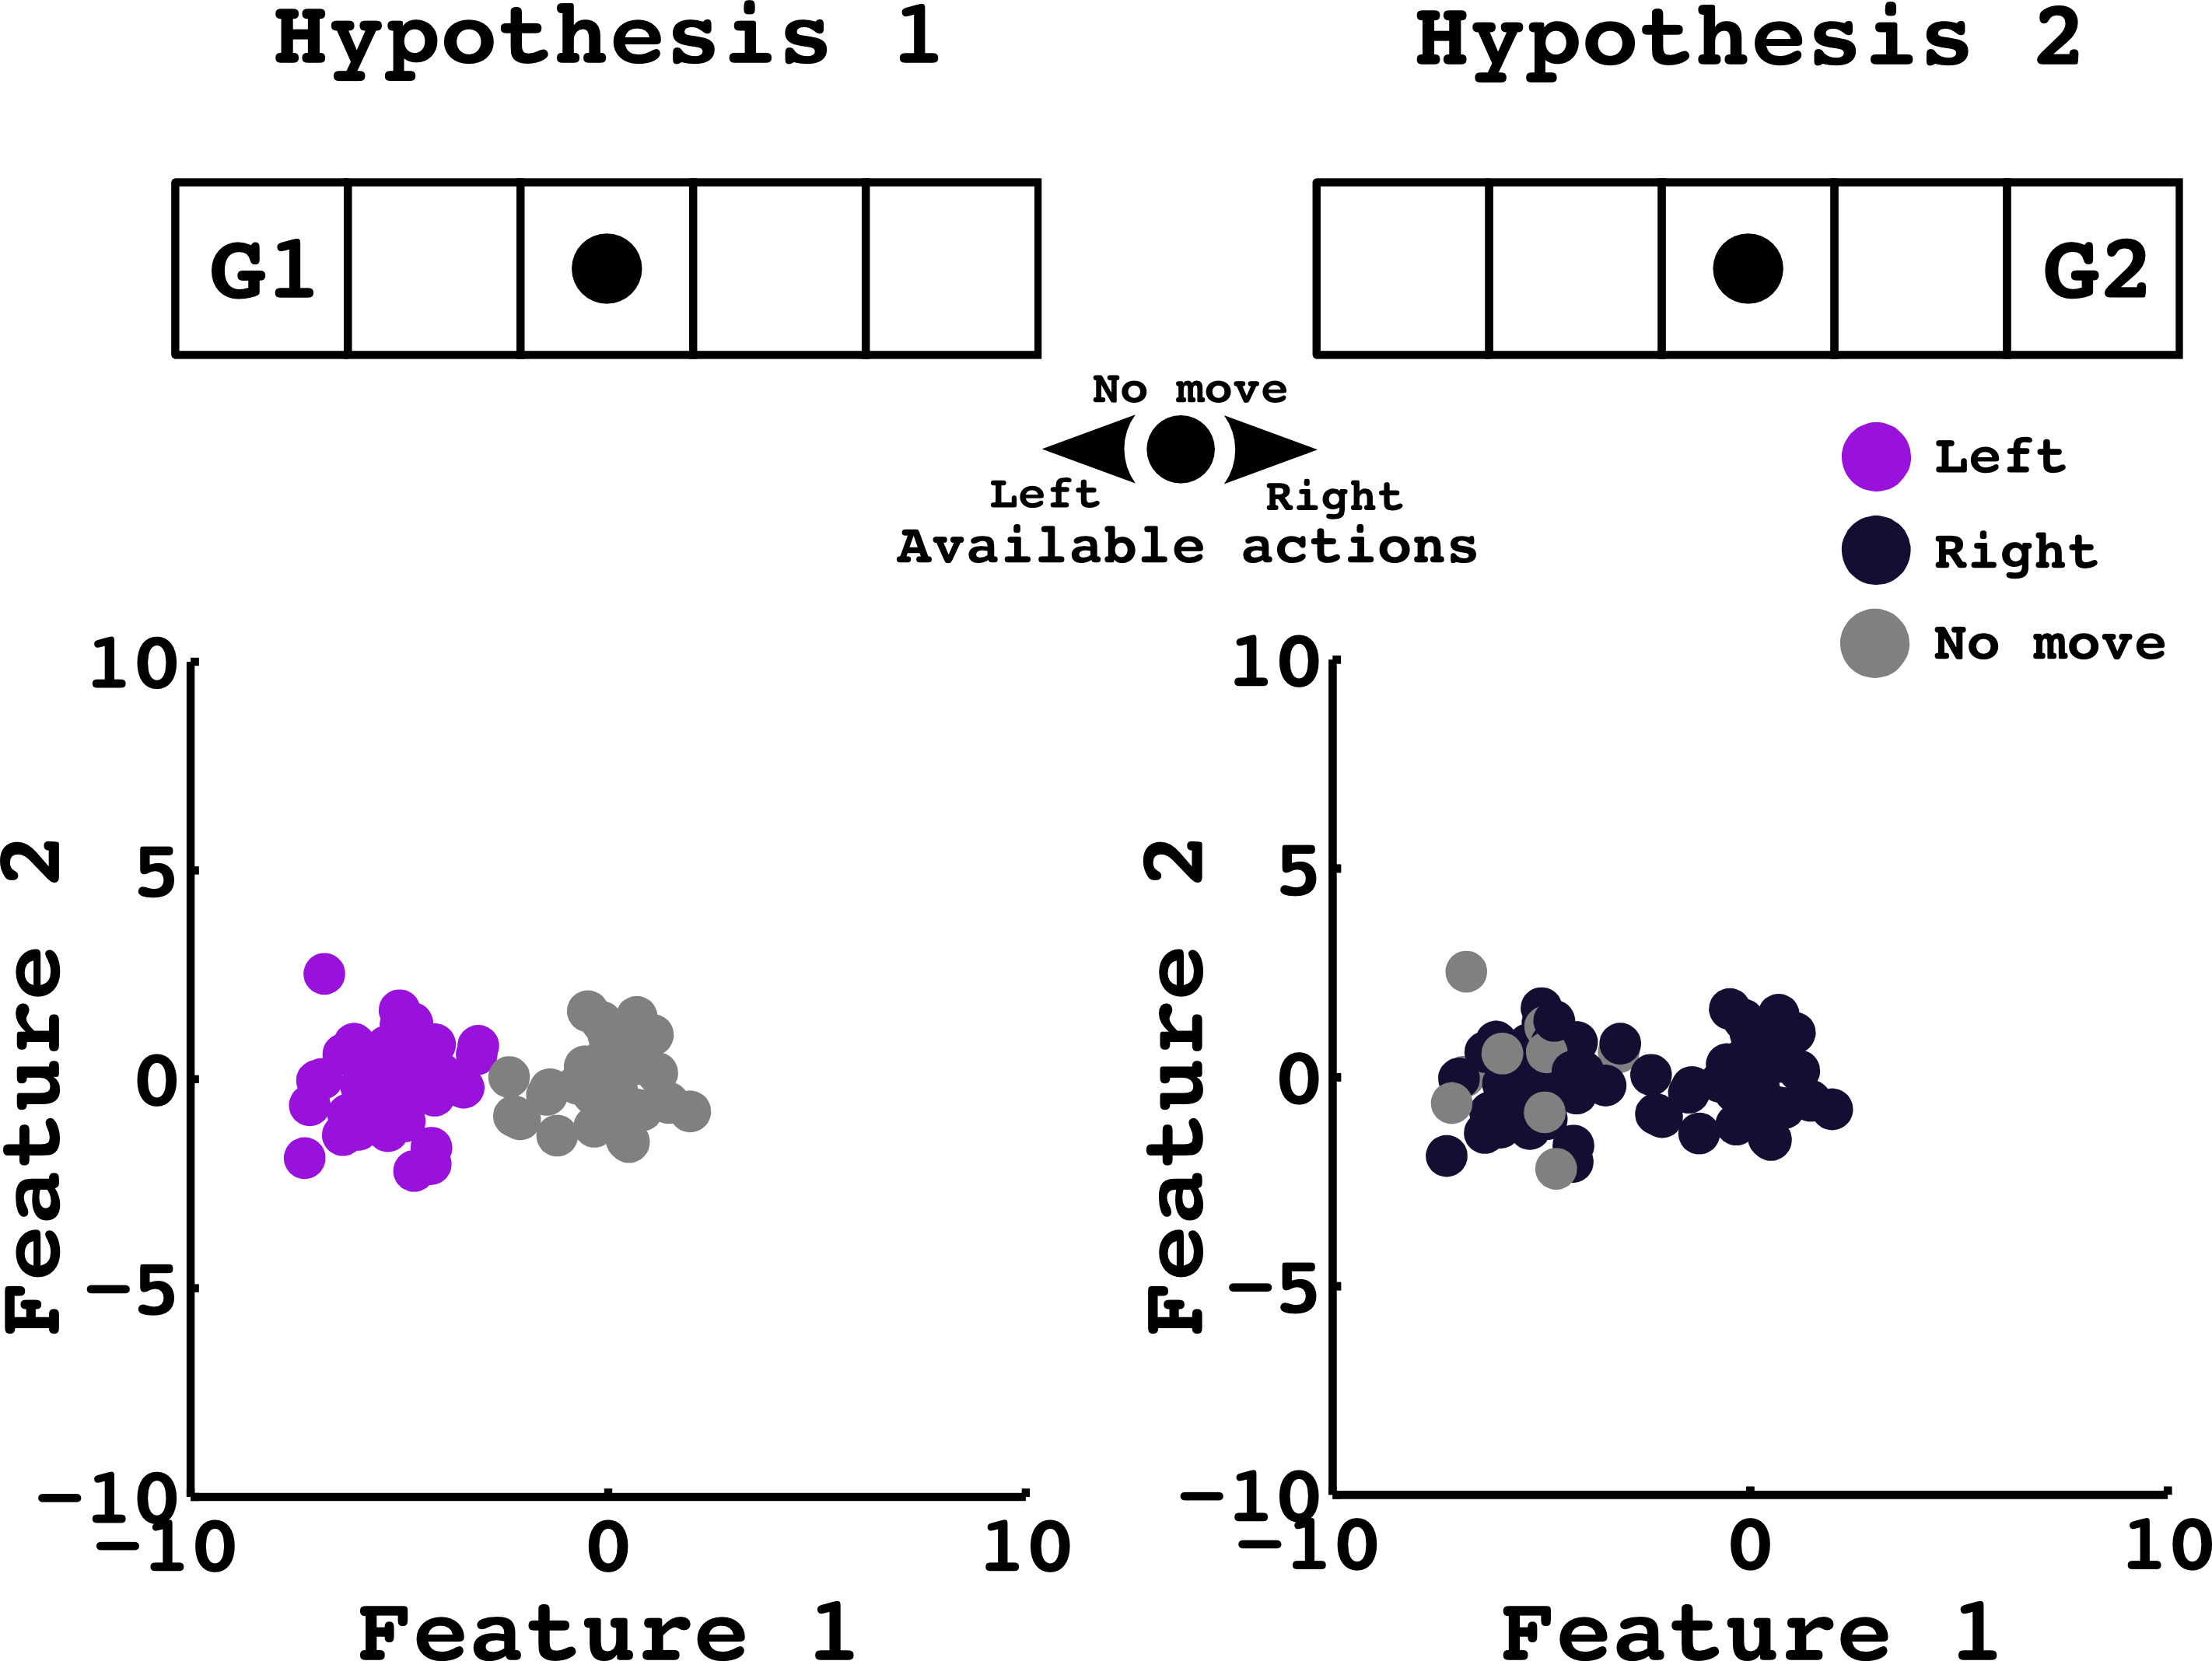
\includegraphics[width=\tworldsize\columnwidth]{\visualspdf/lineworld_symmetries/guidance_3actions.pdf}
  \caption{Interpretation hypothesis for an agent receive feedback on its action in the line word and where hypothetic task are G1 or G2. The agent can perform right, left, or a ``no move'' action. As opposed to Figure~\ref{lineworldguidance2action}, the ``no move'' action allow to break the symmetry of interpretation between G1 and G2.}
  \label{fig:lineworldguidance3action}
\end{figure}

\subsection{Robot's abilities}

We further assume the robot is able to plan its action in order to fulfill a specific task. In other words, if the robot knew what the user wants it to do, it will be able to do it. It implies the robot as full knowledge of the world dynamics and knows how to make a plan. This way the robot can understand the theoretical relation between one action, a specific task and the signal of the user; and therefore create interpretation hypothesis.

However, this ability could have been learn from previous self-exploration session of the environment allowing the robot to learn the dynamics of the environment.

\transition

All those constraints are usually present in the interactive learning literature. 

Some aspects are often more constrained, especially either the signal to meaning mapping is known in advance and the agent infer the task based on the known instructions, either the task itself is known allowing the robot to assign meanings to the teaching signals allowing to it to learn the signal to meaning mapping. Our method generalize over those approach as we neither need to known the task, nor the signal-to-meaning mapping.

Some other constraints are not always applied such as the ability of the robot to plan its action, or the fact that a finite number of task is defined in advance. 

The ability to plan is linked to the need for the robot to evaluate the signals of the user in different situations. To do so it need to be able to project itself in the future to judge of the ``long term'' effect of tis actions. We could considered an agent that has access to the frame but is not able to plan its action in order to fulfill the goal. In such cases, the robot could learn by self-exploration the dynamics of the environment and later use this dynamic to infer a plan for a given task.

The finite set of task hypothesis is a practical constraint for the setup considered in the remaining of this thesis. If the set of task hypothesis was infinite, and considering our interpretation hypothesis approach, we would have to sample a finite number of hypothesis to test on; and given the results, we should re-sample some new hypothesis and test again until some stopping criterion. This process is less reliable than assuming the correct task belong to a finite set of task. It would add an other layer of complexity, hard to track and understand, which would increase the difficult to explain the problem.

The following of this chapter will consider the set of assumptions defined above. In chapter~\ref{chapter:limitations}, we will release the above assumptions, propose solutions to the associated problems and present simple experiments.


%%%%%%%%%%%%%%%%%%%%%%%%%%%%%%%%%%%%%%%%%%%%%%
%%%%%%%%%%%%%%%%%%%%%%%%%%%%%%%%%%%%%%%%%%%%%%
%%%%%%%%%%%%%%%%%%%%%%%%%%%%%%%%%%%%%%%%%%%%%%
%%%%%%%%%%%%%%%%%%%%%%%%%%%%%%%%%%%%%%%%%%%%%%
%%%%%%%%%%%%%%%%%%%%%%%%%%%%%%%%%%%%%%%%%%%%%%
\section{How do we exploit it}
\label{chapter:lfui:how}

As exemplified in Figure~\ref{fig:TworldLabelinterpretation}, generating interpretation hypothesis for each possible allow to find out the task the user has in mind. But as the user have only one objective in mind, only the correct interpretation will correctly assign meanings to the signals. In our example we were able to identify this task visually, by looking at the coherence between the spacial organization of the signals and their associated meanings. But our robots and algorithms, can not use our visual intuition. The key challenge it to find out what measure can reflect the coherence between the spacial organization of the signals and their associated meanings.

A good measure of coherence can be computed by training the classifier on each of the signal-meaning hypothesis pairs and testing its accuracy. As for the wrong hypothesis the signals are not always associated with their correct meanings, it will become impossible to fit a good model on the data. 

By assuming the signals generated by the teacher can be separated by a quadratic curve, and following our example of Figure~\ref{fig:TworldLabelinterpretation}, for each task, we can use the  quadratic discriminant analysis (QDA) \cite{lachenbruch1975discriminant} approach to fit a classifier on the data. For the case of two classes, this classifiers can be represented by two multivariate normal distributions, by  computing the maximum likelihood for the mean and covariance matrix associated to each labels. The results of this process is shown in Figure~\ref{fig:TworldLabelGaussian}.

\begin{figure}[!htbp]
    \centering
    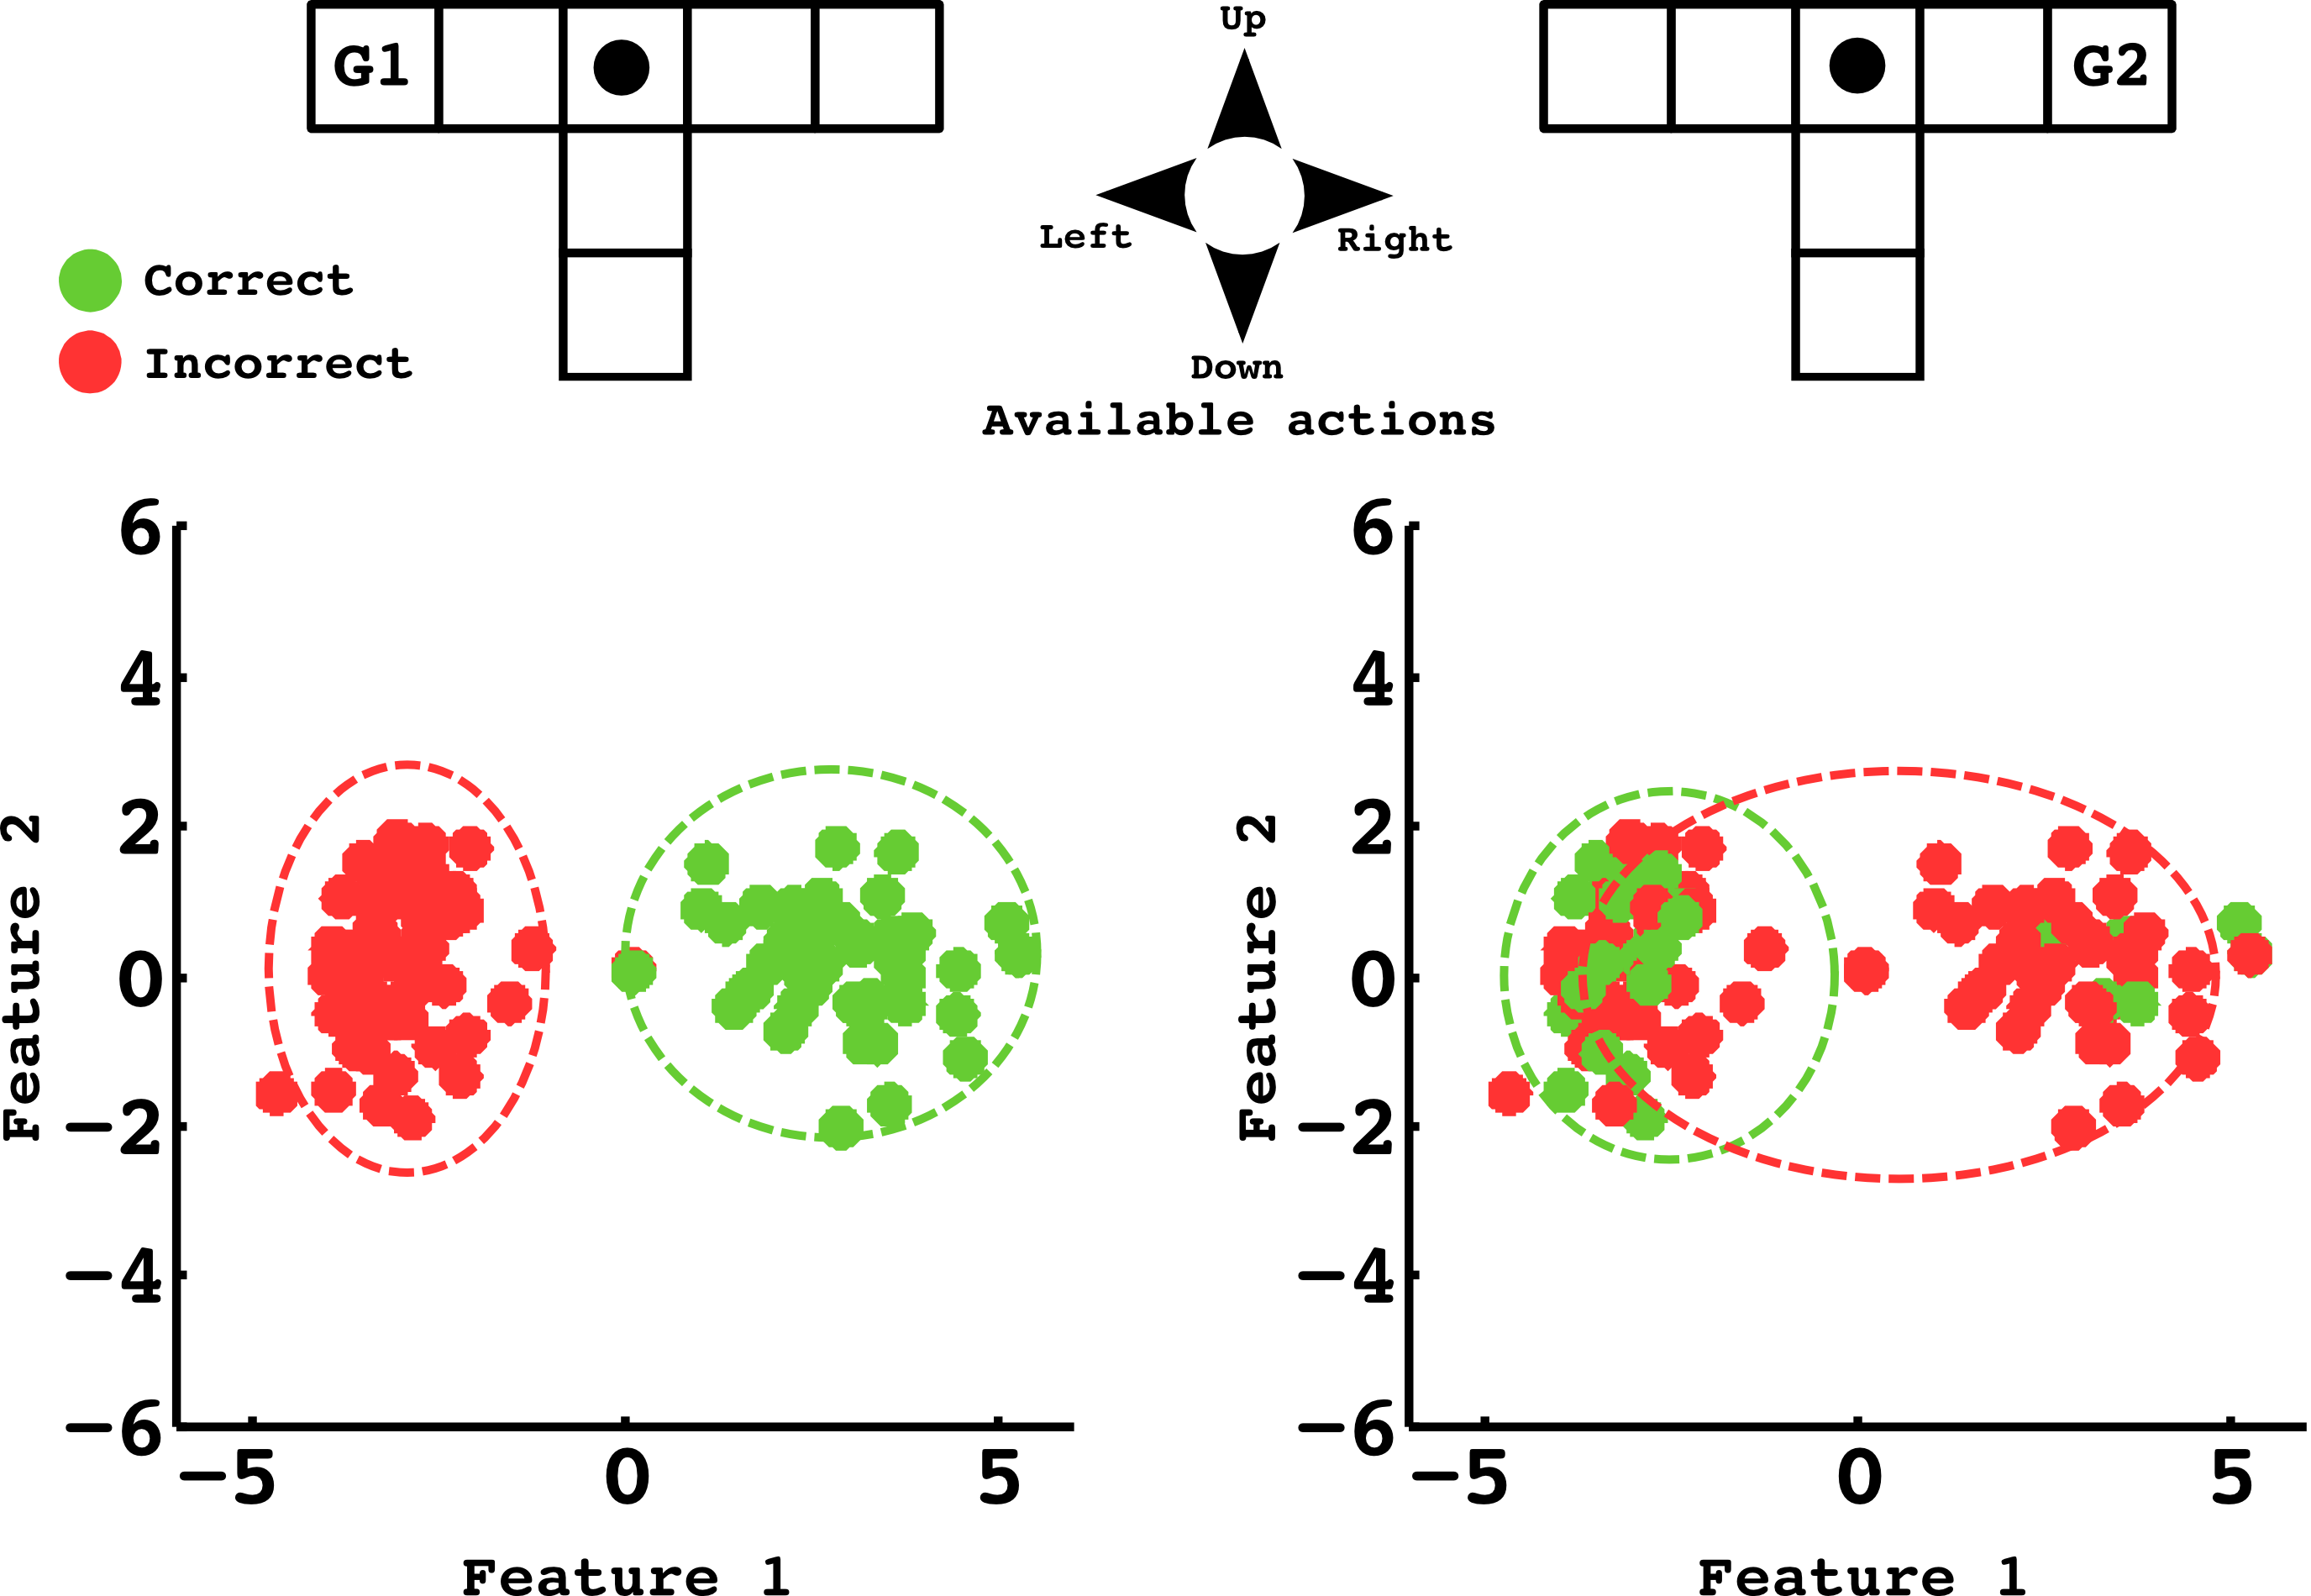
\includegraphics[width=\columnwidth]{\visualspdf/tuto_feedback/Tworld_feedback_labeled_all_actions_with_gaussians.pdf}
    \caption{Interpretation hypothesis made by the agent according to G1 and G2 after many interaction steps with their associated Gaussian distribution (approximated by hand). The teacher's task is to have the agent reach G1. The agent is exploring all the state space randomly. The labels associated to the task G1 are more coherent with the spacial organization of signals in the feature space. This is measured by expected difference in prediction performance made by the each Gaussian classifier.}
    \label{fig:TworldLabelGaussian}
\end{figure}

By computing the performance of the resulting classifiers, we can test which hypothesis satisfies better the assumption that the signals can be separated by a quadratic curve. As stated in the previous section~\ref{chapter:lfui:signalproperties}, here the choice of the classifier encodes in fine our hypothesis on the underlying structure of the data.

The following of this section formalizes this idea and present first results on a pick and place robotic scenario where the user provide instruction using speech utterances. From now on we will use the term label to refer to the meaning associated to user's signals.

\subsection{Notations}

We consider interaction sessions where a machine can perform discrete actions from a set of available actions $a \in \mathcal{A}$ in an either discrete or continuous state space $s \in \mathcal{S}$. The user, that wants to achieve a task $\hat{\xi}$, is providing instructions to the machine using some specific signal $e$, represented as a feature vector  $e \in \mathbf{R}^d$. The task is sequential meaning it is completed by performing a sequence of actions. The machine ignores the task the user has in mind, as well as the actual meaning of each user's signal. Its objective is to simultaneously solve the task and learn a model for the user's signals. To achieve this, it has access to a sequence of triplets in the form $D_M = \{(s_i, a_i, e_i),\ i = 1,\ldots,M\}$, where $s_i$, $a_i$ and $e_i$ represent, respectively, the state, action and instruction signals at time step $i$. The behavior of the machine is determined by the actions $a\in\mathcal{A}$ and the corresponding transition model $p(s'\mid s,a)$.

We assume the system has access to a set of task hypothesis $\xi_1,\ldots,\xi_T$ which includes the task $\hat{\xi}$ the user wants to solve. We assume instruction signals $e$ have a finite and discrete number of meanings $l \in \{l_1, l_2, \ldots, l_L\}$ which we call labels and this is known by the user and the machine. And consider that the agent is given a frame function that given a state $s$, an action $a$ and a task $\xi$ return a label $l$. We will formalize our algorithm in terms of probabilities, therefore the frame represent the conditional probability of a label given a state, action, and a task, written as $p(l | s, a, \xi)$.

Given this frame, the history of interaction $D_M$ and a particular task $\xi$, we can associated with each past signal, given the specific state and action pair the robot was in, a label (or probability of label) resulting in a dataset composed of signal-label pairs. As there is $T$ task hypothesis, we end up with $T$ hypothetic sets. 

We assume that given such a set of signal-label pairs, it is possible to compute a model that classifies signals $e$ into meanings $l$, which we also called the signal to meaning mapping. The parameters of such a model will be denoted by $\theta$. Here again we formalize the classifier as the conditional probability of a label given a signal and a set of parameters, written as $p(l|e,\theta)$.

As the frame and the classifier distribution refers to probabilities about labels, we will use different notation for the labels given by the frame, which we denote $l^f$, and predicted by the classifier, which we denote $l^c$.  Additionally, for a given iteration step $i$, we will superscript our label notation with a $i$ referring to the iteration number.

% For each hypothesis, at time $i$, we have several dataset $D_i^{\xi_t}$, which are used to train a classifier parametrize by $\theta_i^{\xi_t}$. Each classifier $\theta_i^{\xi_t}$ represents an interpretation hypothesis of the user given he is trying to instruct the task $\xi_t$.

\subsection{Estimating Tasks Likelihoods}
\label{chapter:lfui:likelihood}

As explained in the beginning of this section, we will rely on the classification performance of each hypothetic classifier to find out which task is the more likely. More precisely we will compute the probability that every signal is correctly classified given a set of signal-label pairs. It is important to clarify the meaning of correctly classified. Indeed, the agent do not have access to the true labels of the data, so what we mean here by correctly refer to the hypothetic labels given by the hypothetic task considered. In other words, we compute whether or not the classifier computed for the specific state-action pairs is able to separate well the different classes. 

The probability that one signal is correctly classified is the sum across all labels of the probabilities that a signal is of a given label times the probability that the model classifies it as being of this same label. Given an interaction tuple $(s,a,e)$, a task $\xi$, and a classifier $\theta$, we can compute the probability that one signal is correctly classified according to the frame as:
%
\begin{eqnarray}
p(l^c = l^f | s, a, e, \theta, \xi) = \sum_{k = 1, \ldots, L} p(l^c = l_k | e, \theta) p(l^f = l_k | s, a, \xi)
\end{eqnarray}
%
This equation estimate the joint probability for one new iteration step and assume the classifier is already given.  We should now compute the probability that all the labels expected by the frame and all the labels predicted by the classifier match together given a history of interaction and a hypothesized task. Given the full interaction history $D_M$ up to time step $M$, and a task $\xi_t$, we can infer the expected labels $l^f_{1,\ldots,M, \xi_t}$ associated to the signals $e_{1,\ldots,M}$, and compute the associated classifier represented by the set of parameters $\theta_{M, \xi_t}$. 

For clarify of writing we simplify our notations, and remove the $\xi_t$ superscript. It is important for the reader to keep in mind that the robot will never have access to the true intended meaning of the users, therefore, as soon as we infer labels, they are always linked to a hypothesize task, which will always be included in the conditional part of the probability notations. Note that the tuple $(s, a, e)$ are observations independent of the task.

Given the classifier $\theta_M$ associated to the task $\xi_t$ at time step $M$, the probability that every expected and predicted labels match together, which we call the likelihood of the task $\xi_t$, is given by:
%
\begin{eqnarray}
\L(\xi_t) &=& \prod_{i = 1,\ldots,M} p(l^c_i = l^f_i | D_M, \xi_t) \nonumber \\ 
&=& \prod_{i = 1,\ldots,M} \sum_{k = 1, \ldots, L} p(l^c_i = l_k | e_i, \theta_M) p(l^f_i = l_k | s_i, a_i, \xi_t)
\label{eq:matchingoverfitting} 
\end{eqnarray}
%
This equation resumes in computing the odds that all the prediction made by the classifier equals the labels used to train this classifier. Indeed, the classifier $\theta_{M}$ is here computed using all the history of interaction including all the pairs $(e_i, l^f_i)$. This is usually a bad idea to test on data used to learn. Indeed we can already spot a pitfall named overfitting. If the classifier do not generalize and learns a one to one mapping between the provided examples, the above equation will provide the same result for all hypothesis. 

What we really want to test is if the system is able to make correct prediction about what the frame will predict for a new, never observed, situation, i.e. a new tuple $(s,a,e)$. One possible option is to incrementally update the likelihood of each task as soon as new data comes in:
%
\begin{eqnarray}
\L_i(\xi_t) &=& p(l^c_i = l^f_i | D_i, \xi_t) ~~ \L_{i-1}(\xi_t) \nonumber \\ 
&=& \sum_{k = 1, \ldots, L} p(l^c_i = l_k | e_i, \theta_{i-1}) p(l^f_i = l_k | s_i, a_i, \xi_t) ~~ \L_{i-1}(\xi_t) 
\label{eq:matchingfilter} 
\end{eqnarray}
%
where $\theta_{i-1}$ is the classifier trained on all the past observation up to time $i-1$and according to the label generated from task $\xi_t$. And with $\L_{0}(\xi_t)$ being the prior at time 0 (before the experiment starts) for the task $\xi_t$, usually uniform over the task distribution.

While this is a good enough option as it will be demonstrated in the remaining of this thesis, it does not use all available information. Indeed, the update that was made at time $i-10$ is now out of date as we now have $9$ more observation tuple available that may change our past estimates. It would be better to reassess the performance of the classifier given the full set of observation. To do so, and in order to avoid the problem of overfitting, the classifier should be trained on all data but the one tested. We denote by $\theta_{-i}$ a classifier trained on all data available up to time $i$ but the one of time step $i$. We can now rewrite the likelihood as:
%
\begin{eqnarray}
\L(\xi_t) &=& \prod_{i = 1,\ldots,M} p(l^c_i = l^f_i | D_M, \xi_t) \nonumber \\ 
&=& \prod_{i = 1,\ldots,M} \sum_{k = 1, \ldots, L} p(l^c_i = l_k | e_i, \theta_{-i}) p(l^f_i = l_k | s_i, a_i, \xi_t) 
\label{eq:matching} 
\end{eqnarray}
%
While this equation exhibit minor changes over Equation.~\ref{eq:matchingoverfitting}, it avoids problems of overfitting. However, this is already very costly in terms of computational cost and is unlikely to be usable in practice. For example, after $100$ steps, if just $10$ task hypothesis are considered, the system would have to compute $1000$ classifiers to update the likelihoods of each task. While for the previous equations (Eq.\ref{eq:matchingoverfitting,eq:matchingfilter}), if $10$ task hypothesis are considered, we only need to compute $10$ classifiers at each step.

Still, this last approach is not taking into account the quality of the classifier itself before taking into account its prediction. By this we ask the question of knowing how reliable the prediction of the classifier are? A common method to evaluate the uncertainty on the classifier prediction is to use a cross-validation procedure (see chapter~\ref{chapter:introduction:supervised}) to estimate the confusion matrix associated to the classifier. Such confusion matrix allow to infer the conditional probability of one label given the label prediction from the classifier $p(l^{cc} = l_k| l^c = l_q, \theta)$, for every combination of $k$ and $q$ in $1, \ldots, L$. Where $l^{cc}$ is the corrected, or ``temperated'', label predicted by the classifier given our estimates, our past experience, on the quality of its prediction using the cross validation procedure.

For example, a dummy classifier could predict that any given signal $e$ will have a probability $1$ of being of class $l_1$. This classifier is obviously wrong if there more than two labels in the training dataset, and the cross-validation procedure will capture and quantify this problem. If there were 2 classes with equal number of samples, the confusion matrix will give us the following information: $p(l^{cc} = l_1| l^c = l_1, \theta) = p(l^{cc} = l_2| l^c = l_1, \theta) = 0.5$. Meaning that when the classifier predicts label $l_1$ there is $50$ percent chances that the true label is actually $l_1$, and $50$ percent for $l_2$. In other words, the classifier is useless. On the contrary, a perfect classifier, that never makes classification will be represented by the following conditional probabilities: $p(l^{cc} = l_1| l^c = l_1, \theta) = p(l^{cc} = l_2| l^c = l_2, \theta) = 1$ and therefore $p(l^{cc} = l_1| l^c = l_2, \theta) = p(l^{cc} = l_2| l^c = l_1, \theta) = 0$.

We integrate the following measure of prediction uncertainty in equation~\label{eq:matching}:
%
\begin{eqnarray}
\L(\xi_t) &=& \prod_{i = 1,\ldots,M} p(l^{cc}_i = l^f_i | D_M, \xi_t) \nonumber \\ 
&=& \prod_{i = 1,\ldots,M} \sum_{k = 1, \ldots, L} p(l^{cc}_i = l_k | e_i, \theta_{-i}) p(l^f_i = l_k | s_i, a_i, \xi_t)
\label{eq:matchingcrossvalidation} 
\end{eqnarray}
%
with:
%
\begin{eqnarray}
p(l^{cc}_i = l_k | e_i, \theta_{-i}) =  \sum_{q = 1, \ldots, L} p(l^{cc}_i = l_k| l^c_i = l_q, \theta_{-i}) p(l^c_i = l_q | e_i, \theta_{-i})
\label{eq:confusion} 
\end{eqnarray}
%
Those latter equations capture well the full aspect of the problem. However this is extremely time consuming, as it would require to train $10000$ classifiers after $100$ steps, for just $10$ task hypothesis, and using $10$ fold cross-validation. This is impossible to use in real time and, as for Equation~\ref{eq:matchingfilter}, we will rely on an iterative process to cope with this problem:
%
\begin{eqnarray}
\L_i(\xi_t) &=& p(l^{cc}_i = l^f_i | D_i, \xi_t) ~~ \L_{i-1}(\xi_t) \nonumber \\ 
&=& \sum_{k = 1, \ldots, L} p(l^{cc}_i = l_k | e_i, \theta_{i-1}) p(l^f_i = l_k | s_i, a_i, \xi_t) ~~ \L_{i-1}(\xi_t)
\label{eq:matchingfiltercrossvalidation} 
\end{eqnarray}
%
with:
%
\begin{eqnarray}
p(l^{cc}_i = l_k | e_i, \theta_{i-1}) =  \sum_{q = 1, \ldots, L} p(l^{cc}_i = l_k| l^c_i = l_q, \theta_{i-1}) p(l^c_i = l_q | e_i, \theta_{i-1})
\label{eq:confusionfilter} 
\end{eqnarray}
%
where $\theta_{i-1}$ is the classifier trained on all the past observation up to time $i-1$and according to the label generated from task $\xi_t$. And with $\L_{0}(\xi_t)$ being the prior at time 0 (before the experiment starts) for the task $\xi_t$, usually uniform over the task distribution.

Following this latter equation, at each step, for $10$ task hypothesis, and using $10$ fold cross-validation to estimate $p(l^{cc} | l^c, \theta_{i-1})$ the system would have to compute $100$ classifiers to update the likelihoods of each task.

\transition

To summarize, we describe a succession of equation that all measure the same properties of a classifier, namely the probability that all its prediction are correct. We incrementally included some uncertainty measurement to avoid making too sharp estimates when the classifier are known to be of really bad qualities and to avoid the problems of overfitting.

Each term of our pseudo-likelihood is computed from three terms, we will use generic name for the task and the classifier parameter, respectively $\xi$ and $\theta$. $p(l^f|s,a,\xi)$ represents the probability distributions of the meanings according to a task, the executed action and the current state, i.e. it represent the interaction frame. $p(l^c | e, \theta)$ is the raw prediction from the classifier $\theta$. And $p(l^{cc} | l^c, \theta)$ encodes which label should be actually recovered by $\theta$. Intuitively, it models the quality of the model $\theta$.

In practice our pseudo-likelihood is maximized in two steps. First, the maximum a posteriori estimate $\theta$ of each task is computed. Then, the term $p(l^{cc} | l^c, \theta)$ is approximated by the corresponding confusion matrix of the classifier based on a cross validation on the training data. It is the probability that the classifier itself is reliable in its prediction. Finally, the best task $\xi$ should be the one that maximizes the pseudo-likelihood.

Note that the term $p(l^{cc} | l^c, \theta)$ is a global approximation of the uncertainty of the prediction of the classifier. It consider that every predicted signal follow the same ``rule'' and does not depend on the signal $e$ to be predicted. 


% A more precise approach would be to consider a confidence measure on the estimation of each point based on the location of this particular point in the feature space, i.e. $p(l^{cc} | l^c, e, \theta)$. For example, a point that is very close to a bunch of point that all belong to the same class is way more likely to be correctly classified than a point far away from any previously seen point or in the middle of a cloud of point with contradictory labels. For example, Montesano et al. in \cite{montesano2012active} use an algorithm that combines beta–binomial distributions and a non-parametric kernel approach to provide the full distribution for the probability of grasping

\subsection{Decision and Task Change}
\label{chapter:lfui:confidence}

Using any of the equation described above do not inform us about when our system is confident about which task hypothesis is the correct one. Indeed at every iteration step, one likelihood will be higher that the other, but which criteria should we used to decide what value for ``higher'' is enough.

The simplest method is to normalize the likelihood estimates to $1$, and considered the resulting value as the probability of each task:
%
\begin{eqnarray}
p(\xi_t) = \frac{\L(\xi_t)}{\sum_{u = 1,\ldots, T} \L(\xi_u)}
\label{eq:probanormalize} 
\end{eqnarray}
%
Given this measure, we can define a probability threshold $\beta$, and when it exists a $t$ such that $p(\xi_t) > \beta$ we consider task $\xi_t$ is the one taught by the user.

This method suffer from one important drawback, it does not scale well with the number of hypothesis. Indeed, the more hypothesis, the more the difference in likelihood between the best task and the other tasks should be important. Consider for example two cases: \begin{inparaenum}[a)] \item for only two hypothesis whose respective likelihoods are $[0.45, 0.05]$, their normalized likelihood is $[0.9,0.1]$ \item for four hypothesis whose respective likelihoods are $[0.45, 0.05, 0.05, 0.05]$, their normalized likelihoods are $[0.75, 0.083, 0.0833, 0.083]$. \end{inparaenum}. While the difference of likelihood between the best task and the others is the same in both condition, the normalization decreases the importance of the first task with respect to the other. Scaling this to one hundred hypothesis and the normalized likelihood requires huge likelihood difference to reach the same threshold. Normalized likelihood would require to change the threshold for every scenario depending on the number of hypothesis. 

Comparing the likelihood pairwise is a more robust estimate. Considering the example describe above, the first hypothesis was 9 times more likely than all other hypothesis in all condition (2 or 4 hypothesis). We therefore define $W^{\xi_t}$  the minimum of pairwise normalized likelihood between hypothesis $\xi_t$ and each other hypothesis as our measure of confidence:
%
\begin{eqnarray}
W^{\xi_t} = \min_{u~\in~{1, \ldots, T} \smallsetminus \{t\}} \frac{\L(\xi_t)}{\L(\xi_t) + \L(\xi_u)}
\label{eq:probapairwise}
\end{eqnarray}
%
When it exists a $t$ such that $W^{\xi_t}$ exceeds a threshold $\beta \in ]0.5,1]$ we consider task $\xi_t$ is the one taught by the user.

Going back to our previous example: \begin{inparaenum}[a)] \item for only two hypothesis whose respective likelihoods are $[0.45, 0.05]$, their normalized likelihood is $[0.9,0.1]$ while their minimum pairwise normalized likelihood is $[0.9, 0.1]$ \item for four hypothesis whose respective likelihoods are $[0.45, 0.05, 0.05, 0.05]$, their normalized likelihoods are $[0.75, 0.083, 0.0833, 0.083]$ while their minimum pairwise normalized likelihood is $0.9, 0.1, 0.1, 0.1]$. \end{inparaenum}. With our latter measure $W^{\xi_t}$, we can define a threshold that will hold for every scenario independently of the number of hypothesis. 

\subsection{From task to task}
\label{chapter:lfui:tasttotask}

\begin{figure}[!htbp]
  \centering
  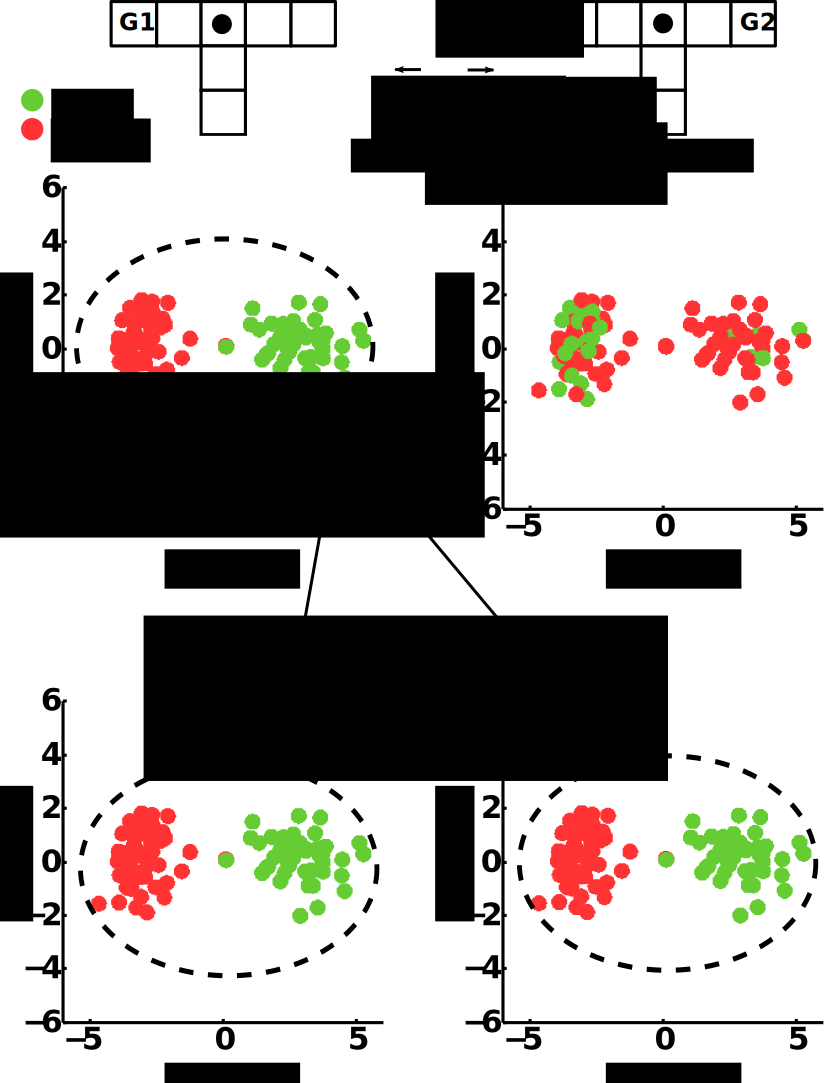
\includegraphics[width=\tworldsize\columnwidth]{\visualspdf/reuse/Tworld_feedback_propagate_labels.pdf}
  \caption{Once a task is identified with confidence, we propagate the label of the best hypothesis to all the other hypothesis.}
  \label{fig:TworldPropagate}
\end{figure}

Once a task is identified with confidence, the robot executes that task and should prepare to receive new instructions from the user to execute a new task. Assuming the user starts teaching a new task using the same kind of signals, we now have much more information about the signal model. Indeed, we are confident that the user was providing instructions related to the previously identified task; therefore we can infer the true labels of the past signals. We can now  assign such labels to all hypothesis (see Figure~\ref{fig:TworldPropagate}) and by using the same algorithm we can start learning the new task faster as all hypothesis now share a common set of signal-label pairs. As described in Figure~\ref{fig:TworldReuse}, the signal to meaning models for each hypothesis are still updated step after step until the new task is identified and labels reassigned.


\begin{figure}[!htbp]
  \centering
  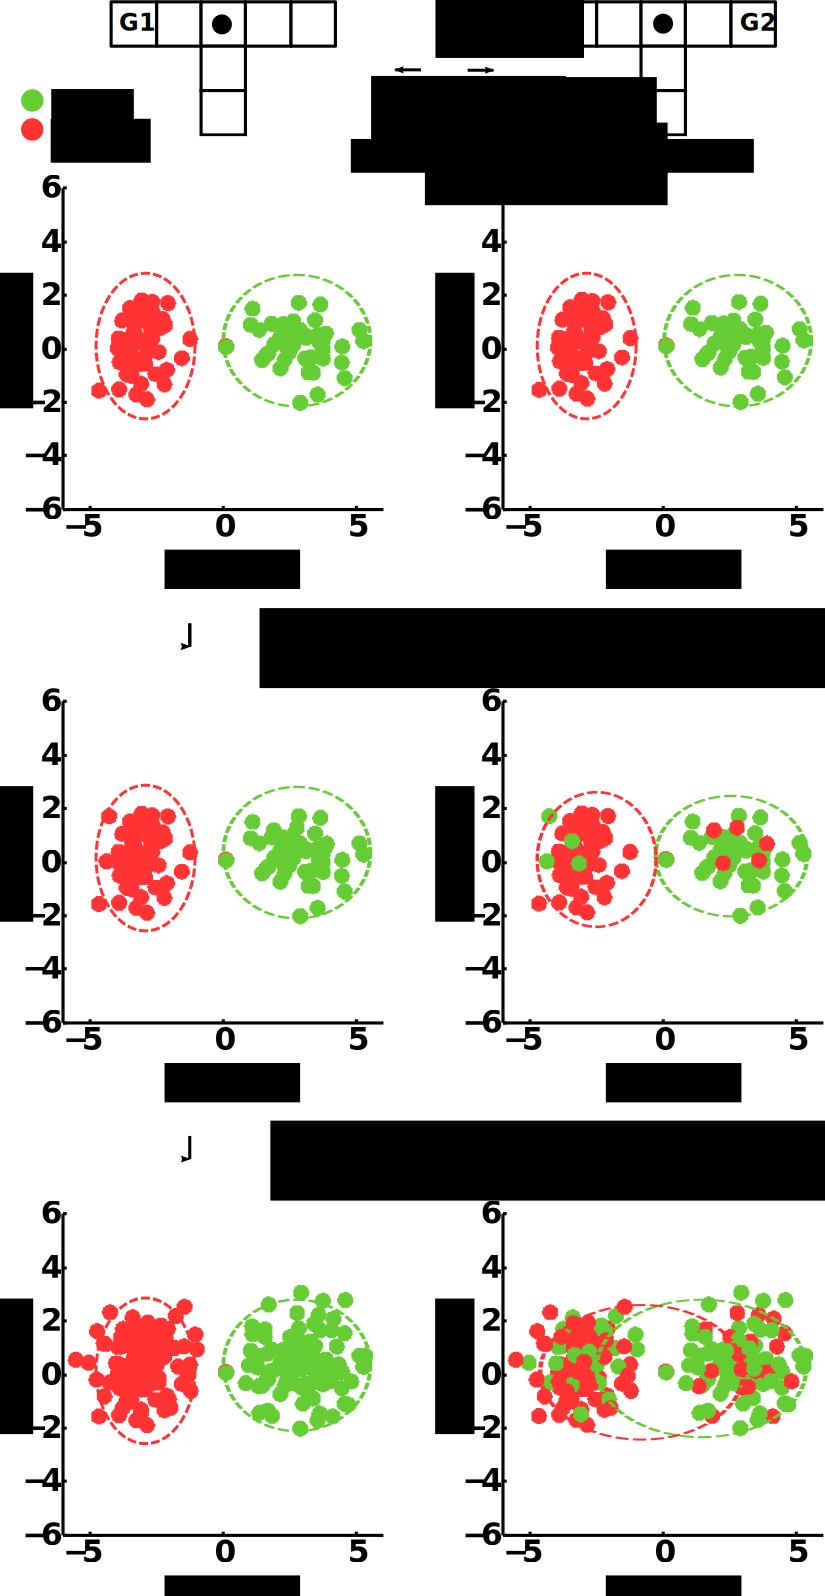
\includegraphics[width=\tworldsize\columnwidth]{\visualspdf/reuse/Tworld_feedback_teaching_again.pdf}
  \caption{When teaching a second task, all hypothesis starts with the same signal-label pairs. After a few new interaction step, some differences in labeling occurs which are easy to detect as they do not comform with the a priori model and allow to discard quickly the second hypothesis G2. But this process also impacts on the trained classifiers which either keep the same quality level or start getting of lower quality for the wrong hypothesis. This is clearly visible after many steps in the new interaction session.}
  \label{fig:TworldReuse}
\end{figure}

This phase of reuse of previous information could be assimlilated to the results of a calibration procedure. Indeed, after a first run we have access to the true intended labels associated to the human signals. However our approach differs in that we keep assigning hypothetic labels for each task and we keep updating the classifier for each task hypothesis. This process allow to decrease the quality of the classifier associated to the wrong hypothesis and helps identifying the correct task faster and more robustly. As examplified in Figure~\ref{fig:TworldReuse}, note that this particular effect is more important for the first few task identified, indeed as the number of shared signal-label pair between hypothesis increases the number of point needed to modify the classifiers increases, and our method therefore converges to a the use of a calibrated classifier shared among all hypothesis. This will be examplified in chapter~\ref{chapter:bci} where we will our method with a standard calibration procedure approach using EEG signals.

\subsection{Using known signals}
\label{chapter:lfui:known}

In some cases the robot may already understand some of the communicative signal from the human. For example, the user could have access to two colored button, one green to mean ``correct'' and one red to mean ``incorrect''. However he may prefer using some speech commands to the robot. To allow for flexible interaction, such speech command should not be preprogrammed as the users may speak different languages, or prefer using the word ``yes'' instead of ``correct'' for example. Considering the mapping between buttons and meanings is known and the mapping between speech utterances and meanings is unknown we can add a terms to our likelihood equations that deal with the known signals. 

Knowing the meaning of a signal resumes in knowing the parameters $\theta_{button}$ corresponding to the mapping between signal and meanings. We can therefore define a separate likelihood update for the known signal that is the same than for the unknown signal, we simply do not update the classifier every step:
%
\begin{eqnarray}
\L_{button}(\xi_t) &=& \prod_{i = 1,\ldots, M} p(l^{cc}_i = l^f_i | s_i, a_i, e_i, \xi_t, \theta_{button})
\end{eqnarray}
%
The likelihood from the speech can be computed using the same process as described in subsection~\ref{chapter:lfui:likelihood}, which we rename $\L_{speech}(\xi_t)$ here for convenience of explanation .

Finally we can compute the final likelihood as the product of estimates from the known signals and from the unknown ones:
%
\begin{eqnarray}
\L(\xi_t) &=& \L_{button}(\xi_t) ~~ \L_{speech}(\xi_t)
\end{eqnarray}
%
It is very important to understand the difference between our method and a more usual method where the signal to meaning mapping is known in advance. This difference lies in the fact we estimate one classifier per task hypothesis depending on the interpretation hypothesis for this specific task. However if we have access to the true signal to meaning mapping, we have only one classifier common to all hypothesis. Therefore all the equation remains the same, only replacing a global classifier by a hypothetic one.

\subsection{Summary and rephrasing}
\label{chapter:lfui:rephrasing}

I would like here to rephrase the ideas developed in this section. The readers that has the feeling of understanding all the aspects of the algorithm can safely skip this section as it is meant to re-explain and summarize the ideas and organization behind the different steps of the algorithm.

The algorithm is divided into a classification algorithm, estimating one classifier for each hypothesis based on past interaction, and a filtering algorithm that uses the results and properties of this classifier to update the belief over hypothesis for current interaction.

The key point is that each hypothesis is believing it is the good one, it is modeling the signal to meaning mapping of the user with respect to each hypothesis objective. We an then testing if this classifier can make accurate prediction on never observed data. As the user is actually following only one hypothesis, and the signal are assumed to have some structure in the feature space, only one hypothesis will be able to predict correctly future interaction. Our assumption is that the hypothesis which shows more coherence between expected label and predicted label is more likely to be the correct one.

To better explain our approach in this section, we will refer to two phases in the learning process: \begin{inparaenum}[a)] \item phase 1 which is learning from scratch a task from unlabeled instructions, and \item phase 2 which is learning a second (or third, or \ldots) task based on the fact we already inferred a first one. \end{inparaenum} Our algorithm is the same for the two phases but different factor are dominating on one or the other learning phase.

Phase 1 is the main contribution of this work and enables a system to be instructed using signal initially unknown. As stated before, our system will generate hypothesis over the possible tasks, infer the hypothetic labels associated to the signal, compute a classifier for each hypothetic set of signal-label pairs, and assume the one of better quality correspond to the one the user has in mind. Bad hypothesis will realize that they are not able to produce coherent output, i.e. to predict properly unseen other signal-label pairs. By doing so the system ends up knowing what is the task taught by the teacher and consequently what are the true labels associated to the teaching signals. Consequently, at the end of phase 1, the system knows a lot more about the mapping between human signals and their meaning.

Phase 2 then seems to be simply learning from known instructions, as we now have the true labels associated to each signals, we can considered the resulting dataset as the result of a calibration procedure. But our algorithm actually improves over this simple approach. After phase one, we do not reduce in the use of one classifier, but we assign the same labels to all hypothesis. The key point is that we keep the hypothesis based approach, which means we keep updating all the classifiers with the new pairs of signal-label from the interaction, interpreted according to each task hypothesis As wrong hypothesis will add wrong signal-label pairs to the classifier, it will reduce the quality of the classifier, therefore reducing the sharpness, and quality, of its prediction; which we take into account in our updates. In other words, we are integrating the fact that the user is not coherent with a hypothesis by integrating new data point, labeled according to the task, in the classifier. Obviously the effect will be quite small if a huge number of samples are already available but we will see in later experiments with brain signals that this process reduces the number of mistakes made by the system, especially when the number of teaching signal is still low.

% In the beginning phase 2, all the classifiers are the same, the difference between hypothesis will be on the match between classified signal and expected label. As we interact with the user, some teaching mistake occurs (\textbf{teaching mistake with respect to the hypothesis considered}) that both create non expected prediction from the classifier and decrease the trust I put into my classifier by mixing labels.

To sum up, the same process is active in both phase. We measure the point based expected classification performance of each classifiers taking into account the classifier intrinsic quality. In the first phase, it is the classifier intrinsic quality that has the most impact as all classifier are very different. In the second phase, it is the expected classifiaction of each individual point that has the most impact, as all classifier share many signal-label pairs, they also share similar classifier and therefore classify the new signals in the same way which either match or mismatch with the expected labels from the frame. The second phase is therefore making sharper decision, as a consequence our method will increase its performances as it keeps interacting with the user.

\transition

In next sections, we present results from our algorithm considering a pick and place robotic scenario where a human wants a robot to build a specific structure and provides instructions to the robot using vocal commands whose meaning are unknown to the robot at start. We present results both in simulation and with a real robotic system where we test different aspects: \begin{inparaenum}[a)] \item learning the associated meaning of instruction words while learning a new task, \item extend it for the case of guidance words, \item combine learning from unknown signals with pre-defined signals of known meanings (buttons), \item reuse learnt signals-to-meaning association for the learning of a new task. \end{inparaenum}

%%%%%%%%%%%%%%%%%%%%%%%%%%%%%%%%%%%%%%%%%%%%%%
%%%%%%%%%%%%%%%%%%%%%%%%%%%%%%%%%%%%%%%%%%%%%%
%%%%%%%%%%%%%%%%%%%%%%%%%%%%%%%%%%%%%%%%%%%%%%
%%%%%%%%%%%%%%%%%%%%%%%%%%%%%%%%%%%%%%%%%%%%%%
%%%%%%%%%%%%%%%%%%%%%%%%%%%%%%%%%%%%%%%%%%%%%%
\section{Method}

We construct a small size pick-and-place task with a real robot. This robot is going to be programmed using a natural speech interface whose words have an unknown meaning and are \textbf{not} transformed into symbols via a voice recognizer. The robot has a prior knowledge about the distribution of possible tasks.

The interaction between the robot and the human is a turn taking social behavior, where the robot performs an action and waits for a feedback, or guidance, instruction to continue. This allows to synchronize a speech wave with its corresponding pair of state and action. The experimental protocol is summarized in figure \ref{fig:lfui:bloc}.

\begin{figure}[!htbp]
  \centering
  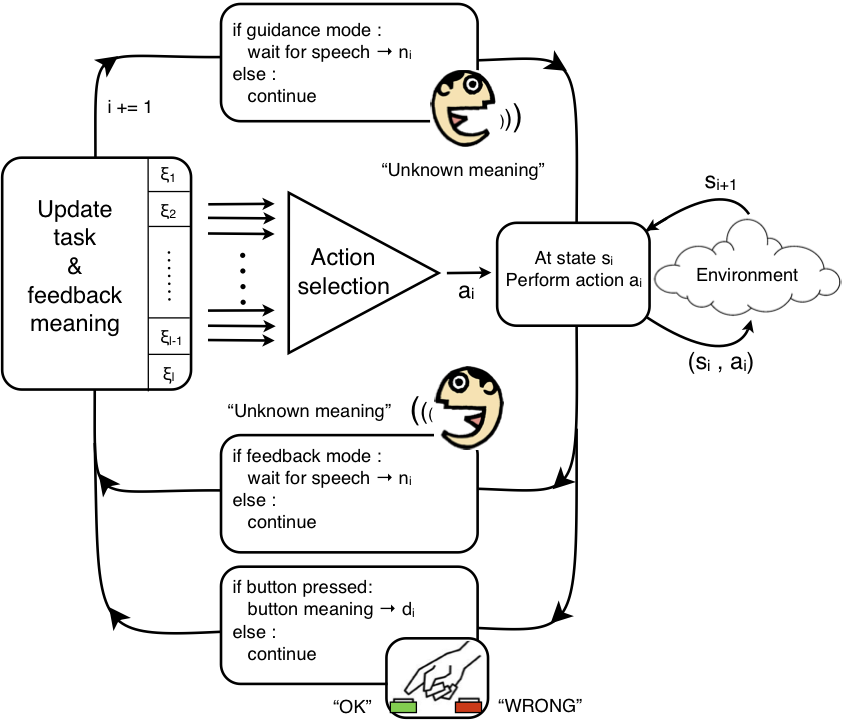
\includegraphics[width=0.6\columnwidth]{\imgpath/bloc.png}
  \caption{Experimental protocol showing the interaction between the teacher and the learning agent. The agent has to learn a task and the meaning of the instructions signals provided by the user, here recorded speech. The teacher can use guidance or feedback signals, and may also have access to buttons of known meanings for the robot.}
  \label{fig:lfui:bloc}    
\end{figure}

\subsection{Robotic System}

We consider a six d.o.f. robotic arm and gripper that is able to grasp, transport and release cubes in four positions. We used a total of three cubes that can form towers of at most two cubes.  The robot has 4 actions available: \textit{rotate left}, \textit{rotate right}, \textit{grasp cube} and \textit{release cube}. The state space is discrete and defined as the location of each object, including being on top of another or in the robot's gripper. For a set of 3 objects we have 624 different states. Figure~\ref{fig:lfui:setup} shows the robot grasping the orange cube. 

\begin{figure}[!htbp]
  \centering
  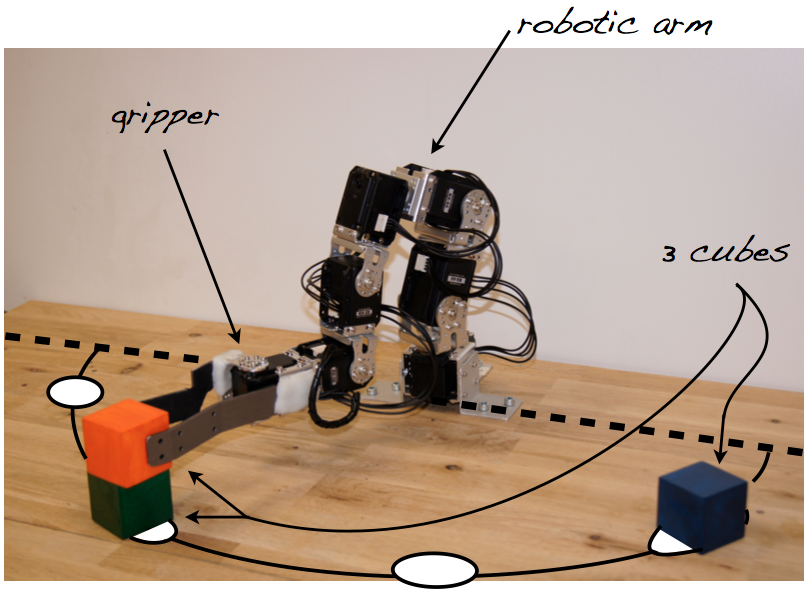
\includegraphics[width=0.5\columnwidth]{\imgpath/setup.png}
  \caption{Robotic System. A six d.o.f robotic arm and gripper learning to performing a pick-and-place task with three cubes.}
  \label{fig:lfui:setup}
\end{figure}

\subsection{Task Representation}

We assume that for a particular task $\xi$ we are able to compute a policy $\pi$ representing the optimal actions to perform in every state. One possibility is to use \textit{Markov Decision Processes} (MDP) to represent the problem \cite{sutton1998reinforcement}. From a given task $\xi$ represented as a reward function we can compute the corresponding policy using, for instance, Value Iteration \cite{sutton1998reinforcement}. In any case, our algorithm does not make any assumption about how tasks are represented.

For this particular representation we assume that the reward function representing the task taught by the human teacher is sparse. In other words the task is to reach one, yet unknown, of the 624 states of the MDP. Therefore we can generate possible tasks by sampling sparse reward functions consisting of a unitary reward in one state and no reward in all the other. 

\subsection{Feedback and Guidance Model}
\label{chapter:lfui:framemodels}

From a given task $\xi$, we can compute the corresponding policy $\pi_{\xi}$. This policy allows to interpret the teaching signals with respect to the interaction protocol defined. In this experiment, we will consider the user is providing either feedback or guidance on the agent's actions. 

\paragraph{} For the feedback case, we define $p(l^f |s,a,\xi)$ as:
%
\begin{equation}
    p(l^f = \emph{correct} |s,a,\xi) = 
    \begin{cases}
    1-\alpha               & if~a = \argmax_a \pi_{\xi}(s,a)\\
        \alpha             & \text{otherwise}\\
   \end{cases}
   \label{eq:feedbackframe}
\end{equation}
%
with $\alpha$ modeling the expected error rate of the user and $p(l^f = wrong |s,a,\xi) = 1 - p(l^f = correct |s,a,\xi)$.

\paragraph{} For the guidance case, the user instructions represent the next action the robot should perform, therefore it only depend on the current state of the robot and the task considered. In our scenario, there is 4 different possible actions ($nA = 4$) in each state. We define $p(l^f |s, \xi)$ for each action as:
%
\begin{equation}
    p(l^f = a |s,\xi) = 
    \begin{cases}
        1-\alpha & if~a = \argmax_a \pi_{\xi}(s,a)\\
        \frac{\alpha}{nA} & \text{otherwise}\\
   \end{cases}
   \label{eq:guidanceframe}
\end{equation}
%
with $\alpha$ modeling the expected error rate. As the agent can perform 4 different actions, we used the constant $\frac{\alpha}{3}$ in order to conserve the property $\sum_a p(l^f = a |s,\xi) = 1$. This assumes the distribution of errors from the teacher are uniform. For those cases where there is more than one optimal action, the probability is uniformly splitted among them. If all actions are optimal, they all share the same probability of $\frac{1}{nA}$.

\paragraph{} It is important to remember that those frames, while capturing a realistic interaction protocol, are arbitrary and we will explicitly ask the user to conform to them. Here we assume the teacher is aware of the optimal policies to fulfill the task, and additionally shares the same representation of the problem than the robot. Especially for the scenario considered, the user should be aware that the robot can not move from position 1 to position 4 in one action. But it should rather pass thought all intermediate position $(1 \rightarrow 2 \rightarrow 3 \rightarrow 4)$. However as we known the user will probably not always provide the good signals, we added a noise term $\alpha$ that account for those unpredictable teaching mistakes. For all following experiments $\alpha$ was set to $0.1$.

But a frame can be way more complex than the simple relation described above. For example, a frame could include the gaze of the user to change the probability that the user is making a mistake. Indeed if the user was looking away from the scene, he is less likely to provide correct feedback. A frame is also not always related to the actions of the agent, it can be that, when the user show an object to the robot, he also spell the name of that object. This frame allows the robot to learn the name of different objects, this frame is often used in language acquisition experiments (see chapter~\ref{chapter:related:language})

\subsection{Speech Processing}
\label{chapter:lfui:speechdata}

We consider speech as the modality for interacting with the robot. After each action we record the teaching word pronounced by the user. This data is mapped into a $20$ dimensional feature space using the methodology described next.  

A classical method for representing sounds is the \textit{Mel-Frequency Cepstral Coefficients} (MFCC) \cite{zheng2001comparison}. It represents a sound as a time sequence of MFCC vectors of dimension $12$. Comparing sounds is done via \textit{Dynamic Time Warping} (DTW) between two sequences of feature vectors \cite{sakoe1978dynamic}. This distance is a measure of similarity that takes into account possible insertions and deletions in the feature sequence and is adapted for comparing sounds of different lengths. Each recorded vocal signal is represented as its DTW distance to a base of 20 pre-defined spoken words which are \textbf{not} part of words used by the teacher.

By empirical tests on recorded speech samples, we estimate that a number of 20 bases words were sufficient and yet a relatively high number of dimensions to deal with a variety of people and speech. This base of 20 words has been randomly selected and is composed of the words:\emph{ \footnotesize{Error, Acquisition, Difficulties, Semantic, Track, Computer, Explored, Distribution, Century, Reinforcement, Almost, Language, Alone, Kinds, Humans, Axons, Primitives, Vision, Nature, Building}}.

\subsection{Classification System for the Instruction Model}

Any machine learning algorithm working for classification problems can be used in our system. This classifier should be able to generalize from the data and have appropriate underlying assumptions on the structure of those data. The rule to choose the classifier is that, if the label were known, the classifier should able to find a good mapping between the signals and their meanings. The only required characteristic is the ability to output a confidence on the class prediction, i.e. $p(l|e, \theta)$.

In this study we decided to compare three classifiers:
\begin{itemize}
\item Gaussian Bayesian Classifier (also called quadratic discriminant analysis (QDA)): Computing the weighted mean $\mu$ and covariance matrix $\Sigma$, the usual equations for Gaussian mixture hold.
\item Support Vector Machine (SVM): Using a RBF kernel with $\sigma = 1000$ and $C = 0.1$. The parameter values have been estimated via a swap of parameters and by estimating performances via a cross validation procedure on the dataset. For SVM probabilistic prediction refer to \cite{platt1999probabilistic}.
\item Linear Logistic Regression: The predictive output value ([0,1]) is used as a measure of confidence.
\end{itemize}

Note that all three classifiers have accuracy close to 100 percent on our speech dataset. This is obviously a quite optimal scenario, we will see in next chapter~\ref{chapter:planning:results} how our algorithm behave with data of poorer quality.

\subsection{Action selection}

The selection of the robot's actions at runtime can be done in different ways. As different sampling methods can lead to different learning behaviors we will compare two different methods: random and  $\epsilon$-greedy. When following random action selection the robot does not use its current knowledge of the task and randomly select actions. Whereas with $\epsilon$-greedy method the robot performs actions according to the current belief of what the task is, i.e. following the policy corresponding to the most likely task hypothesis. The corresponding optimal action is chosen with $1-\epsilon$ probability, otherwise, a random one is selected. In our experiment we show only results with $\epsilon =  0.1$.

It is only in the next chapter that we will investigate how the robot can actively selects its future actions in order to improve its performances.

%%%%%%%%%%%%%%%%%%%%%%%%%%%%%%%%%%%%%%%%%%%%%%
%%%%%%%%%%%%%%%%%%%%%%%%%%%%%%%%%%%%%%%%%%%%%%
%%%%%%%%%%%%%%%%%%%%%%%%%%%%%%%%%%%%%%%%%%%%%%
%%%%%%%%%%%%%%%%%%%%%%%%%%%%%%%%%%%%%%%%%%%%%%
%%%%%%%%%%%%%%%%%%%%%%%%%%%%%%%%%%%%%%%%%%%%%%
\section{Results}
\label{chapter:lfui:results}

Experiments presented in this section follow the protocol described in figure~\ref{fig:lfui:bloc}, where each turn the agent performs one action and waits for the teaching signals from the teacher. We first present a set of simulated experiments using the same MDP as for the real world experiment. We start by assuming that the teacher provides feedback instructions without any mistakes, therefore only the variability in the signals remains. We compare first the different classifiers, and then the performances of $\epsilon$-greedy versus random action selection methods both for feedback and guidance modes. Later, we present an analysis of robustness to teacher mistakes. The last simulated experiment studies the case where the teacher has also access to buttons of known meaning. Finally, we show the result using a real robot where we study how signals knowledge learned in a first run can be used in a second one to learn more efficiently.

In order to be able to compute statistically significant results for the learning algorithm, we created a database of speech signals that can be used in simulated experiments. All results report averages of $20$ executions of the algorithm with different start and goal states. 

As we have $624$ hypothesis, we must update $624$ likelihoods at each step. Depending on the likelihood equation considered this may not be feasible on real time. As we would like to run it in real time and as the speech signal are very well separated int he feature space, we do will use the simplest version of our likelihood estimation method described in Equation~\ref{eq:matchingoverfitting}. To estimate the probability of each task we will normalize the likelihood estimates $\L_(\xi_1),\ldots,\L_(\xi_T)$ to 1.

The interrested reader will find in appendix~\ref{appendix:pickplace} an illustration of the pick and place world as well as the results of the labeling process for the feedback and guidance case.

\subsection{Learning feedback signals}

In this experiment we assume that the robot does not know the words being spoken by the teacher and he does not know the task either. The teacher is providing spoken spoken signals whose meanings are either \texttt{correct} or \texttt{wrong}. The robot will, simultaneously, learn the task and the mapping between the words that are recorded and the binary meanings. The action selection of the robot is done using the $\epsilon$-greedy method. The user uses only one word per meaning.

The results comparing the different classification methods are shown in Figure~\ref{fig:FeedbackOneWord}. It shows the evolution of the probability associated to the task the teacher has in mind. We can track this information because we known, as experimenter, the true task taught, however remember that the robot do not have direct access to this information and should make its decision based on the difference of likelihoods with the other task. Note that after $200$ iterations all three methods identified the correct task as the most likely, i.e. the normalized goal likelihood values for this task are greater than $0.5$, meaning that the sum of all the others is inferior to $0.5$. Logistic regression provides the worse results in terms of convergence rate and variance.

\begin{figure}[!htbp]
  \centering
  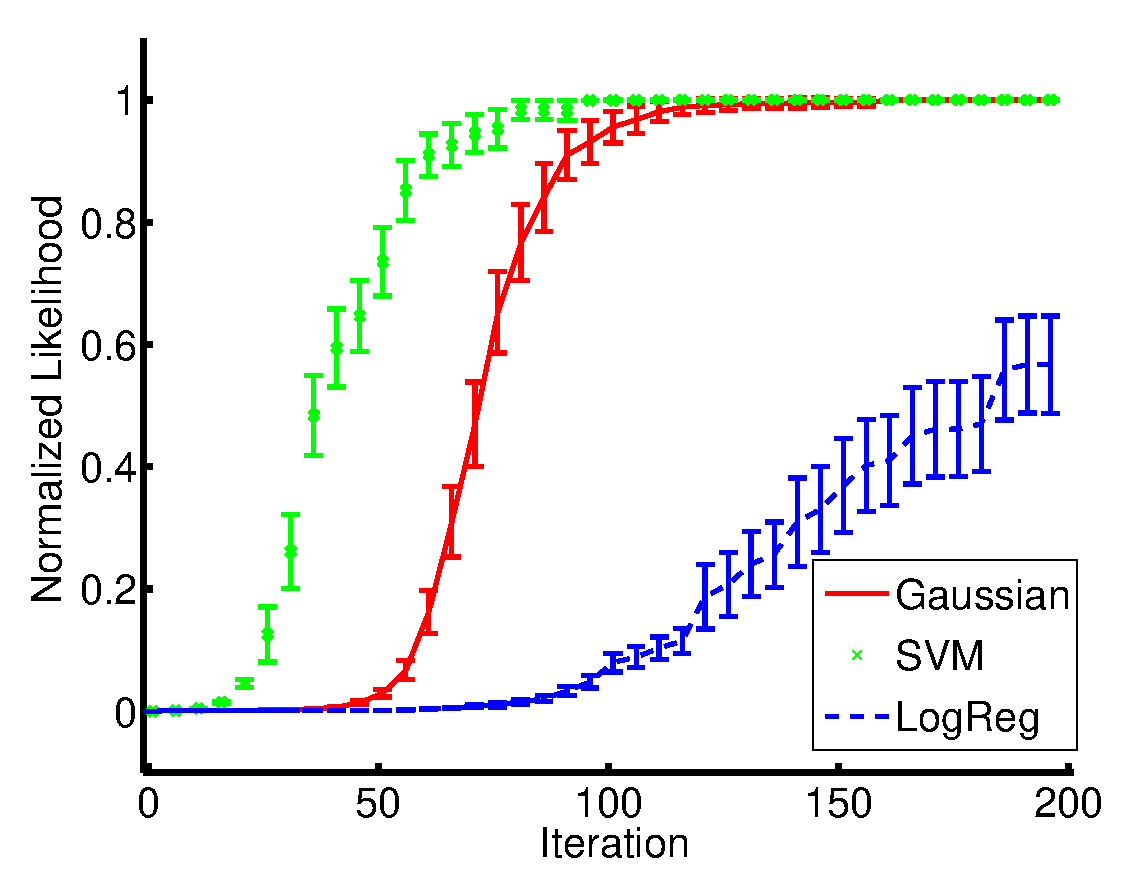
\includegraphics[width=0.7\columnwidth]{\imgpath/classifiers}
  \caption{Taught hypothesis normalized likelihood evolution (mean + standard error) thought iteration using different kinds of classifiers. The teacher is providing feedback using one word per meaning and the agent is performing action according to $\epsilon$-greedy strategy.}
  \label{fig:FeedbackOneWord}
\end{figure}

As soon as the classifier can captures it, the user is not restricted to the use of only one word per meaning. Table~\ref{tab:1} compares the goal normalized likelihood value after $100$ iterations for feedback signals composed of one, three and six spoken words per meaning. SVM has better performance when using one word per meaning but the Gaussian classifier has overall better results with less variance, see Table~\ref{tab:1}. 

\begin{table}[!htbp]
\centering
\begin{tabular}{|l|c|c|c|}
\hline
&\textbf{One word}&\textbf{Three words}&\textbf{Six words}\\\hline
\textbf{Gaussian}&1.0 (0.1)&1.0 (0.1)&0.7 (0.1)\\\hline
\textbf{SVM}&1.0 (0.0)&0.5 (0.4)&0.3 (0.4)\\\hline
\textbf{LogReg}&0.1 (0.1)&0.2 (0.3)&0.2 (0.3)\\\hline
\end{tabular}
\caption{Taught hypothesis normalized likelihood values after 100 iterations (mean and standard deviation). Comparison for different classifiers and number of words per meaning. The Gaussian classifier has overall better performances.}
\label{tab:1}
\end{table}

Interestingly the Gaussian classifier learns better after $100$ iterations than the other classifiers with many words per meaning. This counter intuitive result can be explain by the high dimensionality of the space where even one Gaussian can differentiate several groups of clusters. Linear logistic regression have lower performance presumably due to the linear decision boundary. For the SVM classifier, which is kernalized, as only 100 data points are distributed between each cluster, the more the number of cluster increase the less data point per cluster. The iterative fitting process of the SVM is therefore more likely to consider some data as noise, omitting some clusters. For the following experiments, we will only consider the Gaussian classifier, first because it has overall better performance but also because it is the faster to train and thus is the only one usable for real world and real time experiments. Indeed, in this setup, at each iteration the agent has to train $624$ classifiers.

\subsection{Learning guidance signals}

In Figure~\ref{fig:Guidance}, we compare the performance of learning from unknown feedback or unknown guidance signals. Between feedback and guidance method, the number of meanings is increased from two (correct/incorrect) to four (left/right/grasp/release). As with feedback, the robot is able to identify the task based on guidance signals but need more iterations to reach a perfect knowledge. This may seem counter intuitive as for the guidance case the robot receives more informative signals. However it now needs to classify instructions in four meanings which requires more samples to identify the clusters. 

\begin{figure}[!htbp]
  \centering
  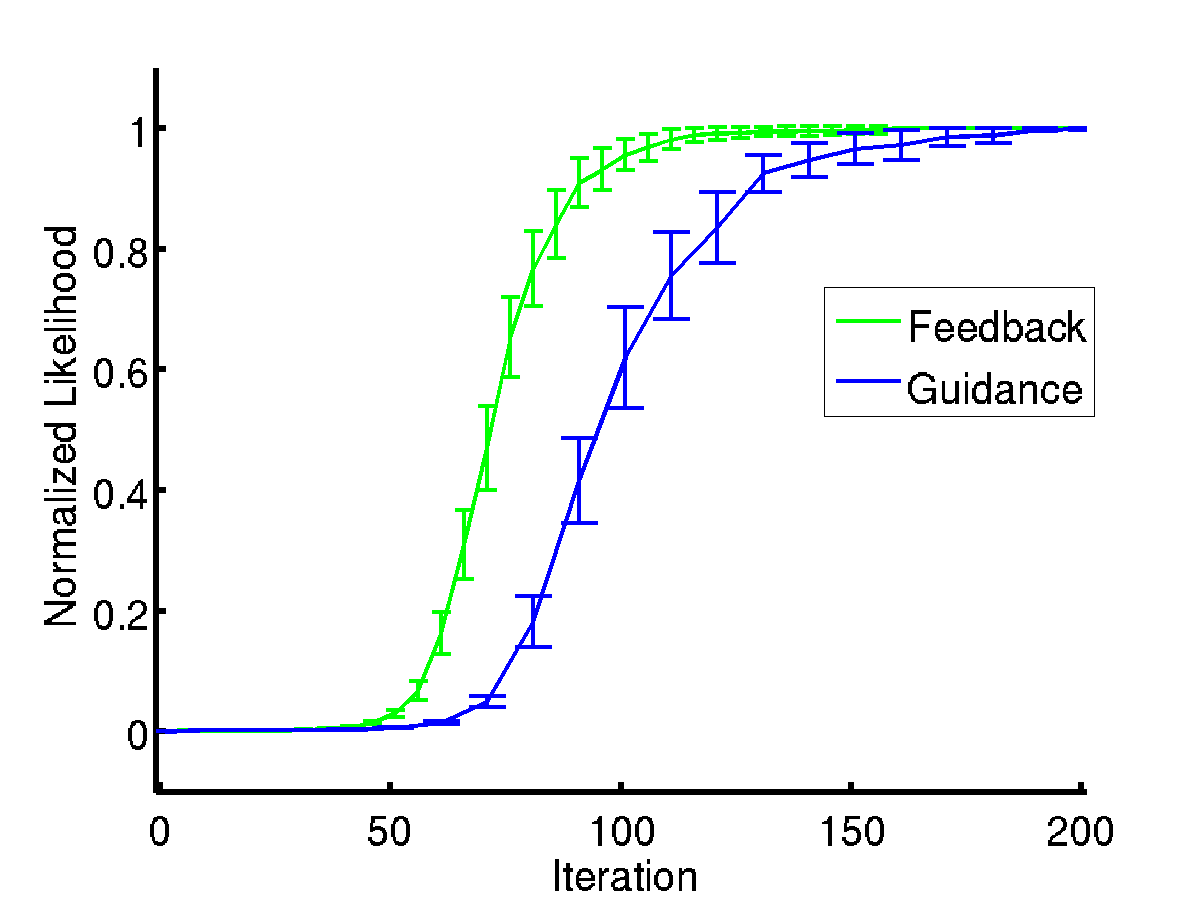
\includegraphics[width=0.7\columnwidth]{\imgpath/feedback_vs_guidance}
  \caption{Taught hypothesis normalized likelihood evolution (mean + standard error) thought iteration using Gaussian classifier. Comparison of feedback (green) and guidance (blue) instructions using one word per meaning. The robot is able to learn the task based on both feedback and guidance signals but needs more iterations to reach a perfect knowledge for the guidance case.}
  \label{fig:Guidance}
\end{figure}

\subsection{Robustness to teaching mistakes}

In the results presented until now, we made the assumption that the teacher is providing feedback or guidance signals without any mistake. But real world interactions are not perfect and people can fail in providing correct feedback. That is why we included the $alpha$ constant in our frame's equations (see section~\ref{chapter:lfui:framemodels}
). An analysis of robustness is shown in figure~\ref{fig:Noise} using feedback signals, Gaussian classifier and one word per meaning. We compares two way of training the Gaussian classifiers: \begin{inparaenum}[a)] \item estimating the maximum likelihood (ML) of the Gaussian for each class, namely the mean and covariance, and \item using the expectation maximization (EM) algorithm to iteratively update the mean and covariance of each class in order to find the underlying structure of the data. \end{inparaenum} 

We show that the EM approach is improving robustness to teaching mistakes as it allows to find the true underlying structure more efficiently. Referring to our previous discussion in section~\ref{chapter:lfui:whynotEM}, note that we initialized the EM algorithm with the ML estimates for each Gaussian and tracked which Gaussian belongs to which meaning. In addition the representation use for the spoken words makes them well separated in the feature space and it is unlikely that the EM algorithm fails at finding the two clusters given the data properties.

\begin{figure}[!htbp]
  \centering
  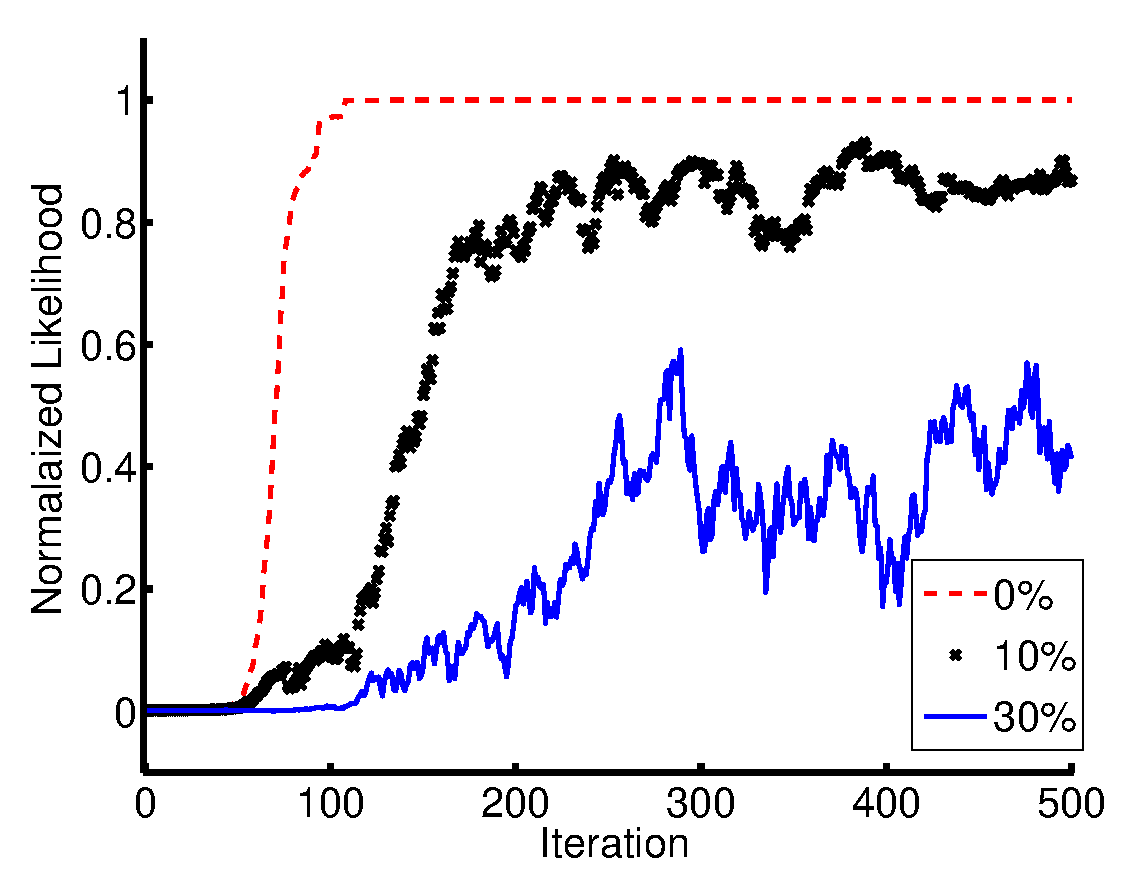
\includegraphics[width=0.49\columnwidth]{\imgpath/noise_no_EM}
  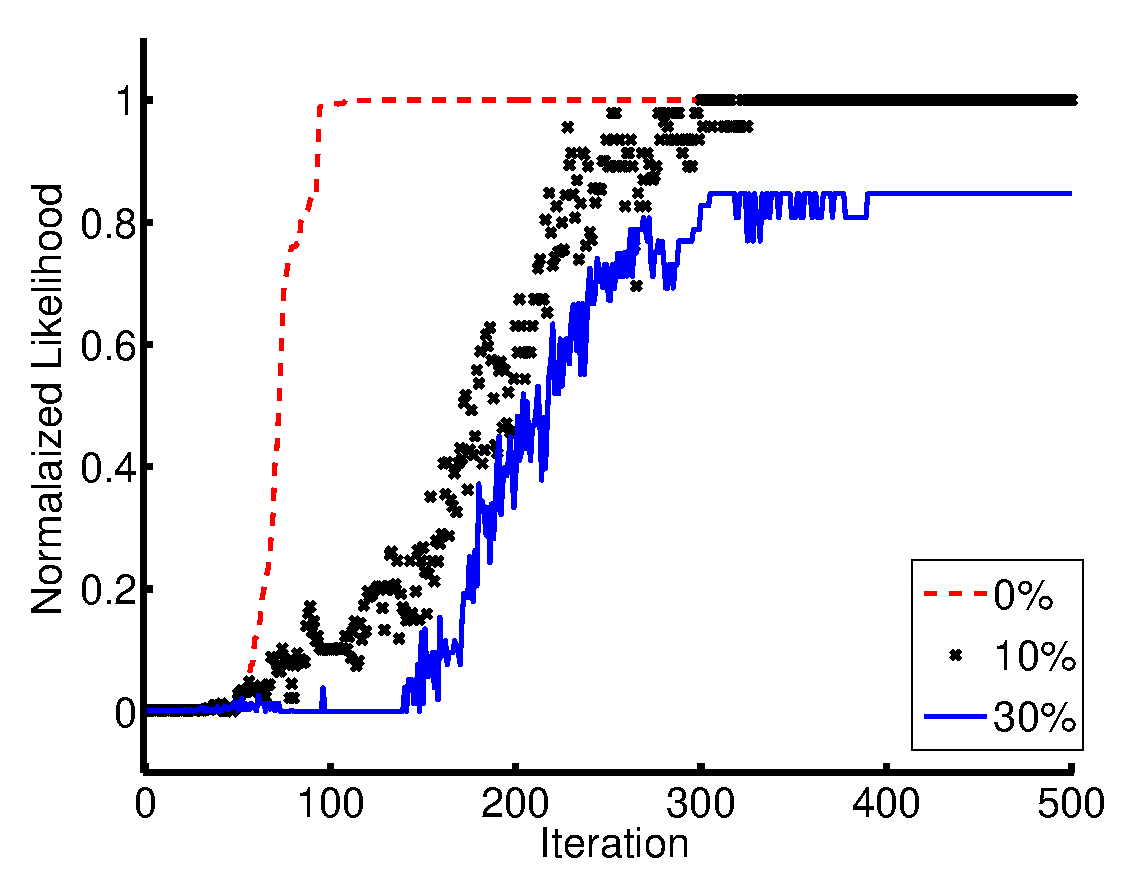
\includegraphics[width=0.49\columnwidth]{\imgpath/noise_with_EM}
  \caption{Taught hypothesis normalized likelihood evolution thought iteration using Gaussian classifier. Comparison of the ML estimates (left) versus EM estimates (right). The teacher is providing feedback using one word per meaning with different percentage of mistakes. $\epsilon$-greedy action selection. Standard error has been omitted for readability reason.}
  \label{fig:Noise}
\end{figure}

\subsection{Including prior information}
\label{sec:IncludingPriorInformation}

Learning purely from unknown teaching signals is challenging for the researcher but could be restrictive for the teacher. Therefore sources of known feedback could be added, such as a green and a red button, where the green button has a predefined association with a ``correct'' feedback meaning, as red button with a ``incorrect'' meaning. Yet, we shall expect that even in this case, users will use more modalities than the predefined one.  

In this study, the teacher still provides initially unknown spoken words feedback but can also use the red and green button as described in figure~\ref{fig:lfui:bloc}. However, and in order to avoid the possibility of direct button to signal association, it can never use both modalities at the same time and use them alternatively with equal probability. Therefore, in average, after 250 iterations the robot has received 125 known feedback and 125 unknown speech signals. In most systems half of the information would be ignored but our method enable learning from the unknown signals. We study three learning methods: in the first case, the robot is learning only via the known feedback, i.e. the buttons; in the second it uses only the vocal unknown signal; and in the third one, it uses both. Figure~\ref{fig:button} shows result from this setting. 

\begin{figure}[!htbp]
  \centering
  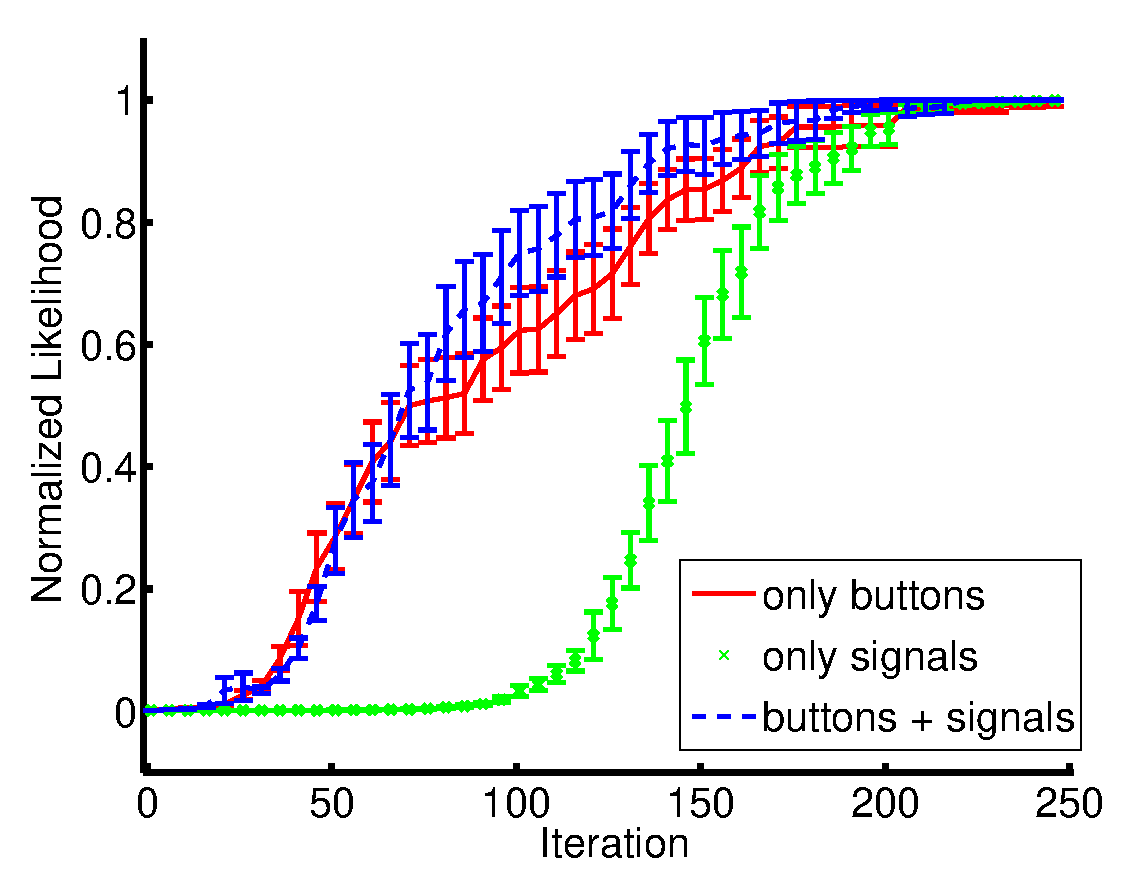
\includegraphics[width=0.7\columnwidth]{\imgpath/mix_button}
  \caption{Taught hypothesis normalized likelihood evolution (mean + standard error) thought iteration using Gaussian classifier. Comparison of using known button, unknown signals and both.}
  \label{fig:button}
\end{figure}

As expected, learning from known feedback is faster than with unknown, however taking advantage of different sources of information, even a priori unknown, can led to slightly better performances than using only known information. Importantly, the signals to meaning knowledge of the robot is updated and could therefore be reused in further interaction.

\subsubsection{Reuse using a real robot}

Statistical simulations have shown that our algorithm allows an agent to learn a task from unknown feedback in a limited amount of interactions. To bridge the gap of simulation we tested our algorithm in real interaction conditions with our robotic arm. In this experiment, the teacher is facing the robot and chooses a specific goal to reach (i.e. a specific arrangement of cubes he wants the robot to build). He then decides one word to use as positive feedback and one as negative feedback and starts to teach the robot. For this experiment the word \textit{``yes''} and \textit{``no''} were respectively used for the meaning ``correct'' and ``incorrect''. 

Once the run is terminated we keep in memory the classifier corresponding to the best task, i.e. having the higher likelihood value, and start a new experiment where the human teacher is going to use the same feedback signals to teach a new task. But this time the spoken words are first classified as ``correct'' or ``incorrect'' meaning according to the previously learnt classifier. Therefore we can use the same method are when learning from the buttons. We study here two things, first does our system bridges the reality gap and can we reuse information learnt from a previous experience? 

Figure~\ref{fig:Real} shows results from this setting. In the first run it takes about $100$ iterations for the robot to learn the task. Whereas in the second run, when reusing knowledge from the first one, the robot is able to learn a new task faster, in about $30$ iterations, meaning that it has well found the two clusters in our $\mathbb{R}^{20}$ dimensional space as well as the mapping to their corresponding meaning. I was the user for this studies and was aware of the task representation used by the robot, i.e. a MDP with four discrete actions. As explained in chapter~\ref{chapter:related:humanintheloop} an important challenge is to deal with non-expert humans whose teaching styles can vary considerably. However this challenge is not part of the current study and we observed that different non-informed users teaching the robot had different understanding of the robot behaviors which led to unsuccessful interactions.

\begin{figure}[!htbp]
  \centering
  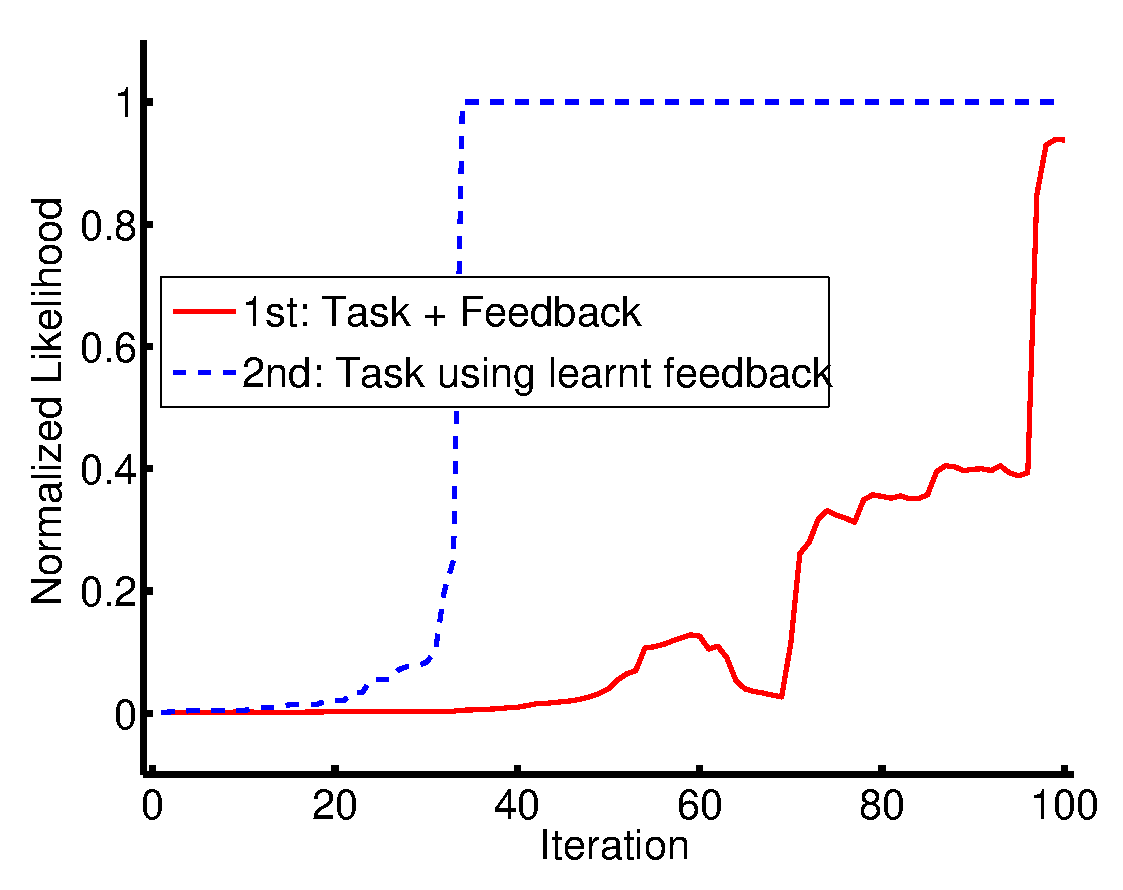
\includegraphics[width=0.7\columnwidth]{\imgpath/real}
  \caption{Taught hypothesis normalized likelihood evolution thought iteration using Gaussian classifier.  Feedback using one word per action. $\epsilon$-greedy action selection. A first run of $100$ iterations is performed where the robot learns a task from unknown feedback. Then by freezing the classifier corresponding to the best task estimate, the user teaches the robot a new task.}
  \label{fig:Real}
\end{figure}

This experiment was done at a very early stage of this work and was not yet considering the method discussed in section~\ref{chapter:lfui:tasttotask}, but only a simplified version were the label from the first task are used to calibrate a classifier used for the learning of the second task.

\subsection{Action selection methods}

Finally we compare the impact of using different action selection methods, we consider $\epsilon$-greedy and random action selection methods.

Figure~\ref{fig:selectionMethod} left and right compares respectively the action selection method for the case of feedback and guidance interaction frames. The $\epsilon$-greedy method results in a faster learning with less variance. This method, at each step, leads the robot in the direction of the most probable goal. In this way it will receive more diverse feedback and will visit more relevant states than what a random exploration would do.

\begin{figure}[!htbp]
  \centering
  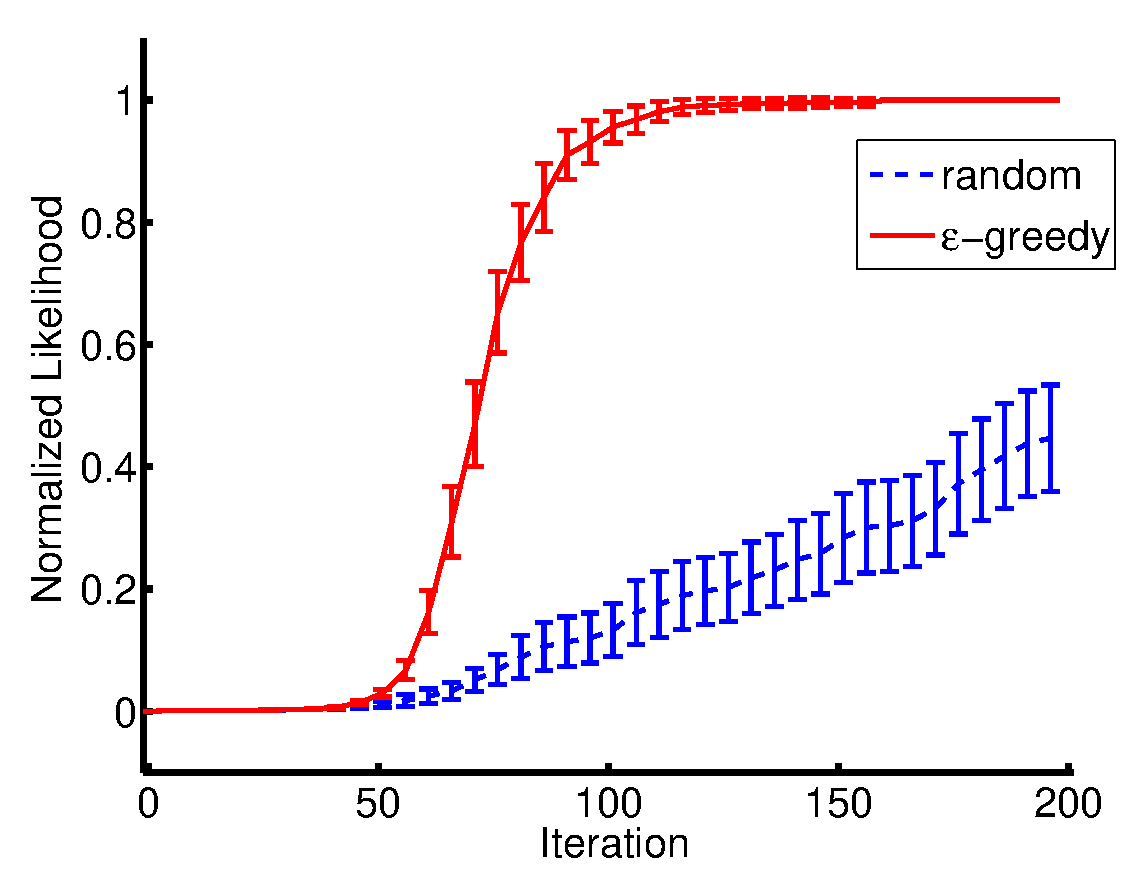
\includegraphics[width=0.49\columnwidth]{\imgpath/feedback}
  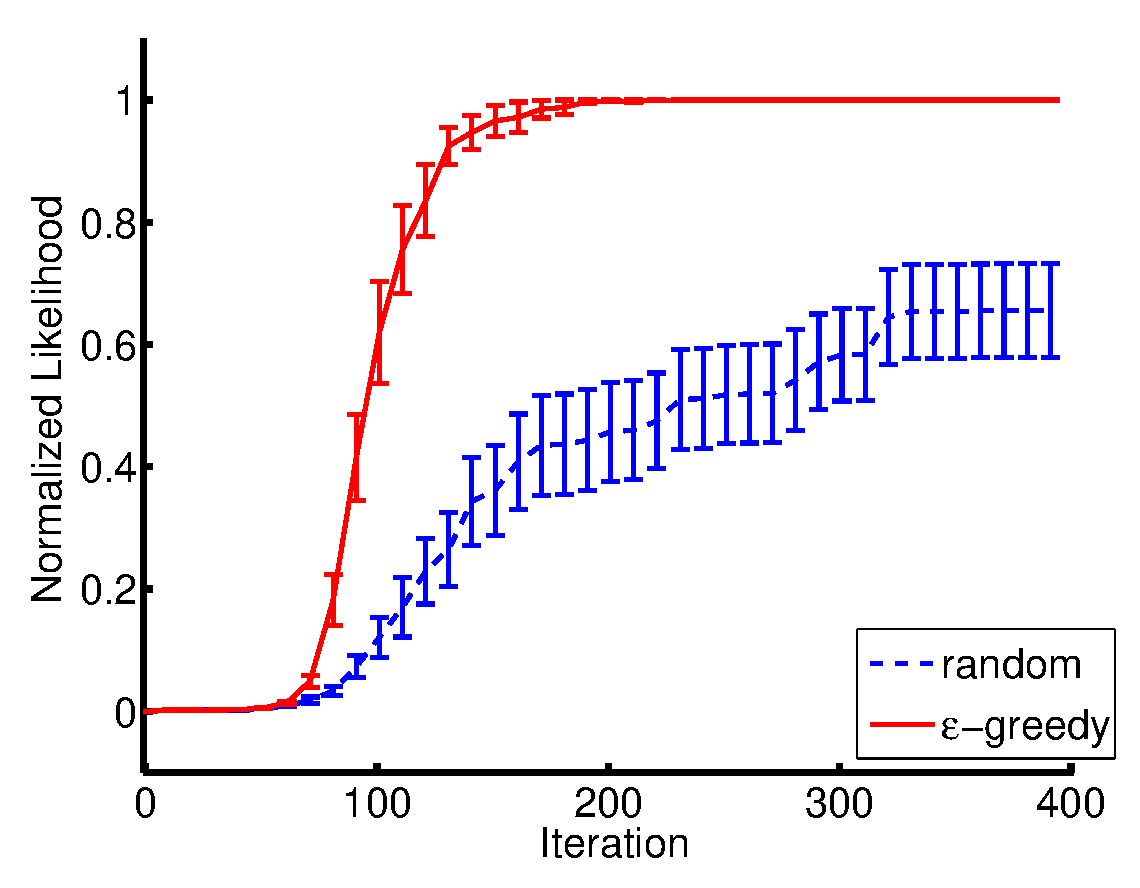
\includegraphics[width=0.49\columnwidth]{\imgpath/guidance}
  \caption{Taught hypothesis normalized likelihood evolution (mean + standard error) thought iteration using Gaussian classifier. The teacher is providing feedback (left) or guidance (right) signals using one word per meaning. The $\epsilon$-greedy action selection method learns faster than the random one. Note that the x-axis showing the number of iteration from start does not considered the same range.}
  \label{fig:selectionMethod}
\end{figure}


\transition

We showed that learning simultaneously a task and the meaning of an a priori unknown human instruction is possible and that the action selection method impacted the learning performances. Can we do better than random or $epsilon$-greedy action selection method? 

Using an active learning approach \cite{settles2010active}, it should be more time efficient to choose the actions that are expected to reduce the uncertainty as fast as possible. In next section we will investigate and details the specific aspect of the uncertainty in our setting, where not only the task is unknown but also the signal to meaning mapping. We will provide measures of uncertainty that can be used as exploration bonus for planning exploration strategies. And present results from artificial dataset of different qualities in a two-dimensional grid world.

%%%%%%%%%%%%%%%%%%%%%%%%%%%%%%%%%%%%%%%%%%%%%%
%%%%%%%%%%%%%%%%%%%%%%%%%%%%%%%%%%%%%%%%%%%%%%
%%%%%%%%%%%%%%%%%%%%%%%%%%%%%%%%%%%%%%%%%%%%%%
%%%%%%%%%%%%%%%%%%%%%%%%%%%%%%%%%%%%%%%%%%%%%%
%%%%%%%%%%%%%%%%%%%%%%%%%%%%%%%%%%%%%%%%%%%%%%
% \section{Discussion}

% In this work we presented an interactive learning system that can learn the initially unknown association between unlabeled instruction signals and their meaning while learning a new task. We presented empirical results showing that 1) our system can learn from unknown feedback, unknown guidance instruction signals, or a mixture of these signals, 2) it can recover from teaching mistakes, 3) it can leverage additional known sources of information, and 4) different standard classifiers can be used. An experiment with a real robot and a real user showed that 5) it can reuse acquired knowledge about human instruction signals in the learning of a new task. Finally we presented an extended experiment that mixed unknown feedback and guidance instructions, in a continuous environment, and showed that 6) an uncertainty based planning algorithm, using uncertainty from both task estimation and instruction classification, is the most efficient strategy.

% \subsection{Instruction modalities} Instruction signals were here conveyed using speech sounds (which may have been interjections, or even sounds of clapping or tapping hands). Of particular interest is the possibility to use the same system with multiple modalities for instruction signals, such as facial expressions or hand gestures. This allows different users to use the system according to their own modality preferences, potentially related to their own skills and limitations. In principle, since no part of the system is specific to the sound modality, and since the sound modality is already relatively complex, there are no theoretical obstacle for this experimental extension. An interesting example might be to consider brain-computer interfaces system \cite{chavarriaga2010learning, iturrate2010robot} that usually require a long an explicit training phase. Using our system we would be able to simultaneously understand the meaning of brain signals and what task is the user trying to achieve. We started investigating in that direction with promising preliminary results \cite{grizou2013zero}.


% say that the signal were very easy to classify




